\subsection{Relevamiento de requerimientos Generales}

\subsubsection{Objetivos y requerimientos a cumplir}

Para lograr tener uns visi�n intencional del sistema, tanto en su parte funcional como en la no funcional, presentamos los objetivos que identificamos organizandolos en un Diagrama de Objetivos\footnote{Objetivos organizados en uno o mas arboles, donde tenemos que casa objetivos se logra gracias al cumplimiento de los objetivos dependientes (hijos inmediatos)}

{\large Diagrama de Objetivos \label{fig:doCasino}}
\begin{center}
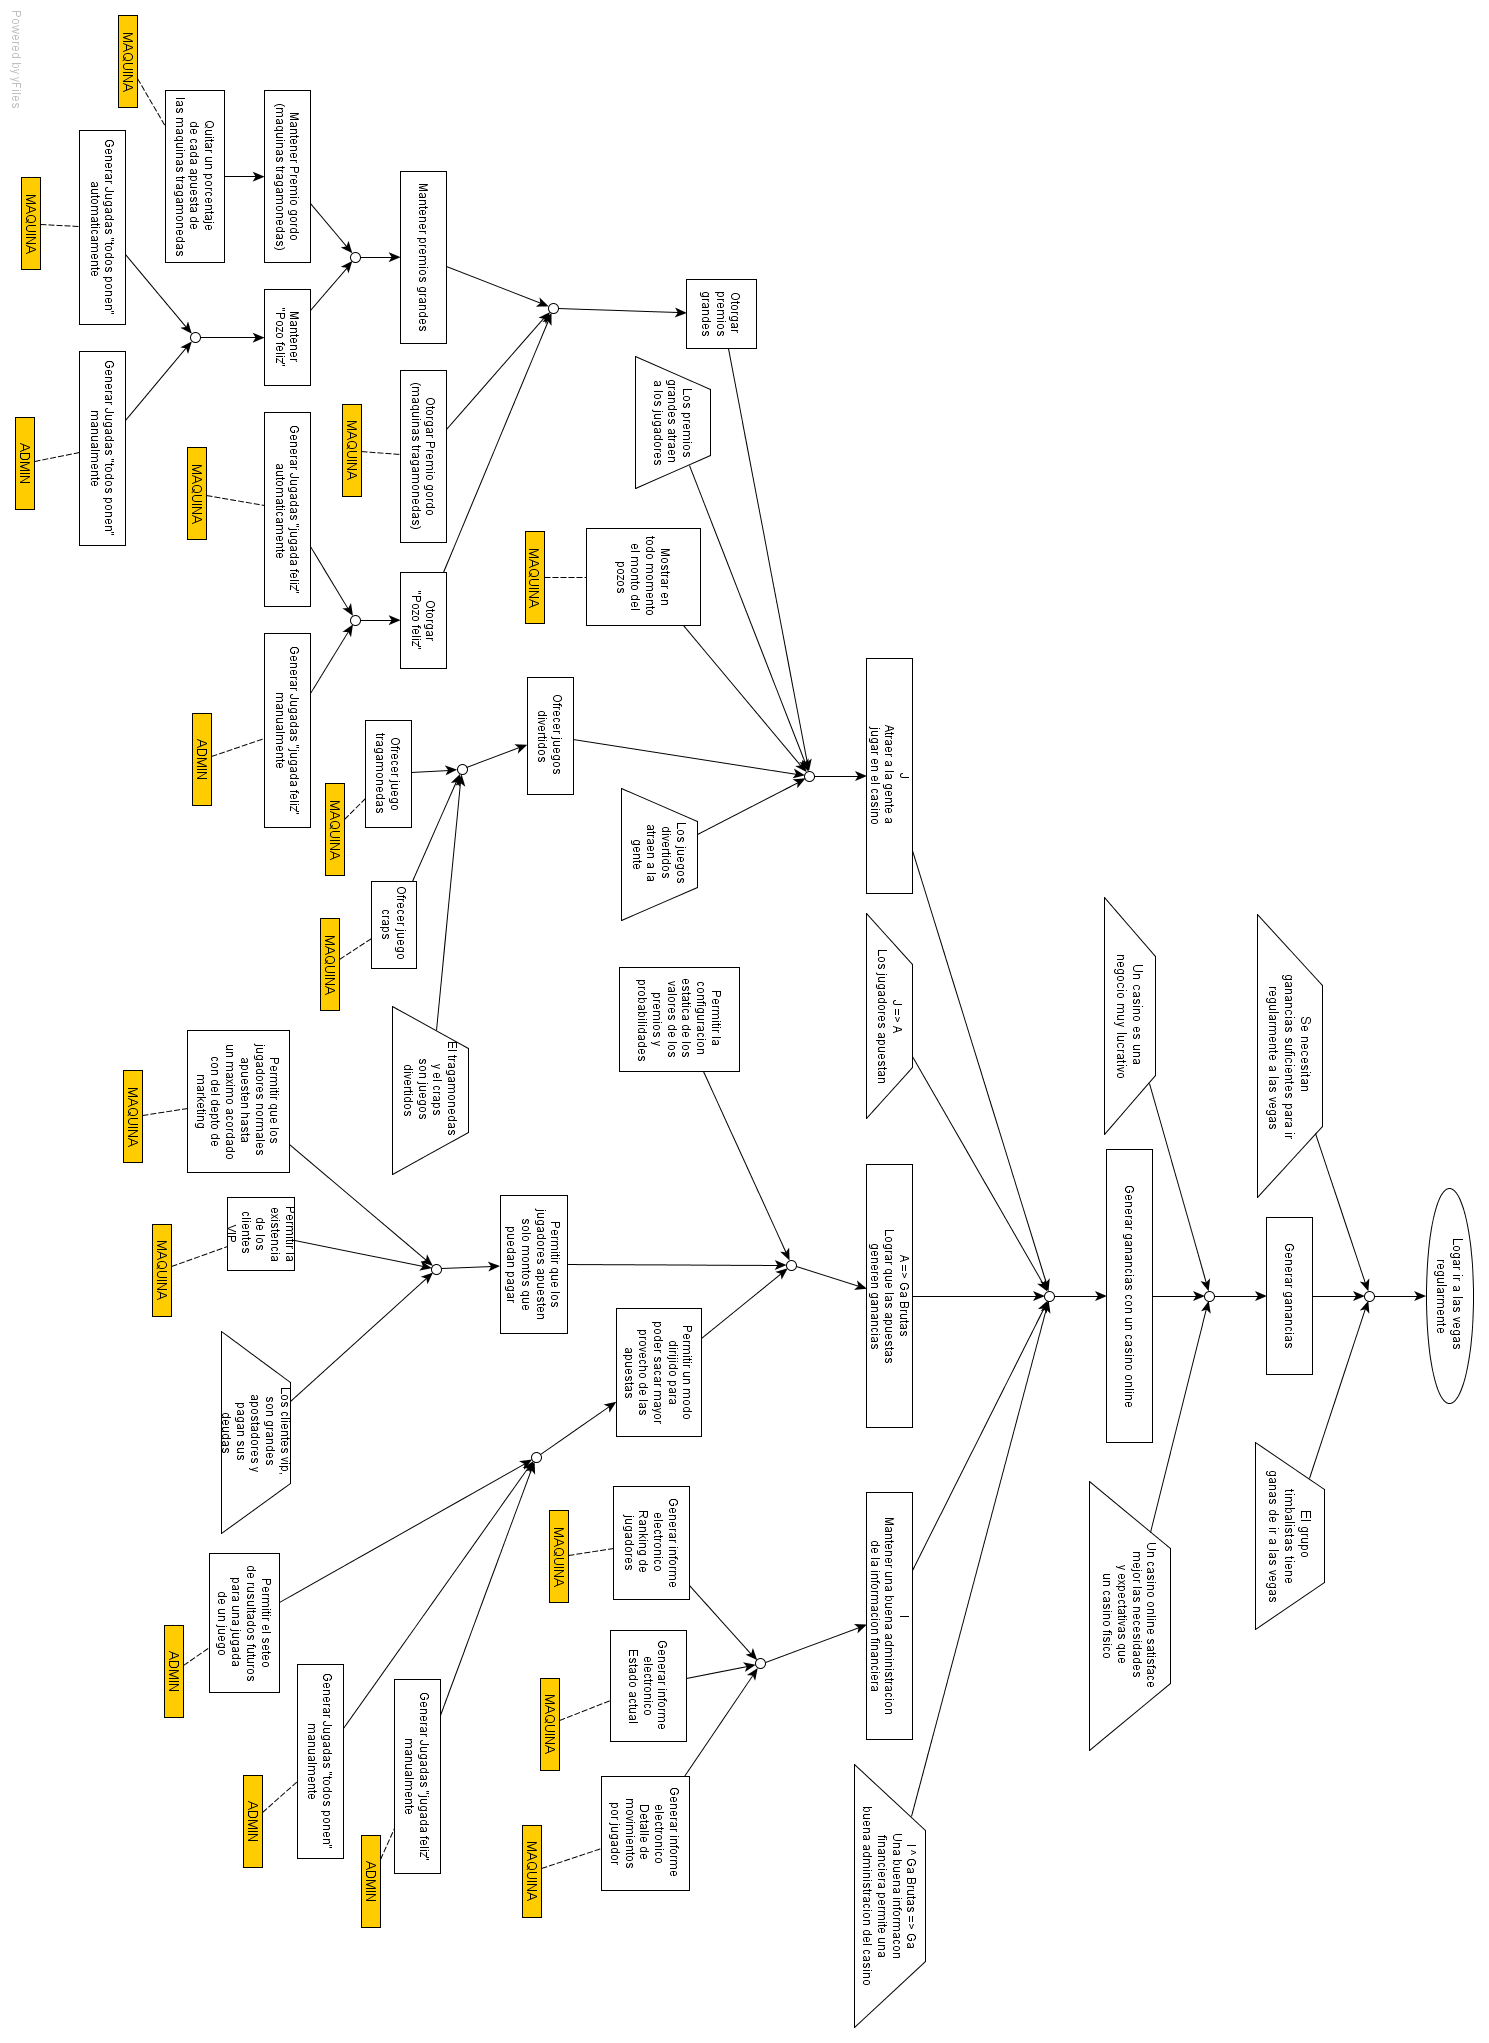
\includegraphics[scale=0.25]{img/doCasino.png}
\end{center}

\begin{framed}

\depto Con este Diagrama de Objetivos intentamos dar el primer paso en la definicion del alcance del sistema y la justificacion de los requerimientos encontrados.
Tambien sera de utilidad para el analisis de los supuestos sobre los que se basar� el sistema.

\end{framed}

\subsection{Analisis de agentes involucrados en el sistema}

Para comprender mejor la manera en que deberan relacionarse los distintos sujetos del mundo con el sistema a construir y sus interacciones, estucturamos el mundo con un Diagrama de contexto\footnote{Diagrama de contexto: Diagrama donde las cajas son agentes activos del sistema y las flechas son las interacciones basicas}

Este diagrama tambien nos da otra mirada del alcance y expectativas del software a construir.

{\large Diagrama de Contexto \label{fig:dcCasino}}
\begin{center}
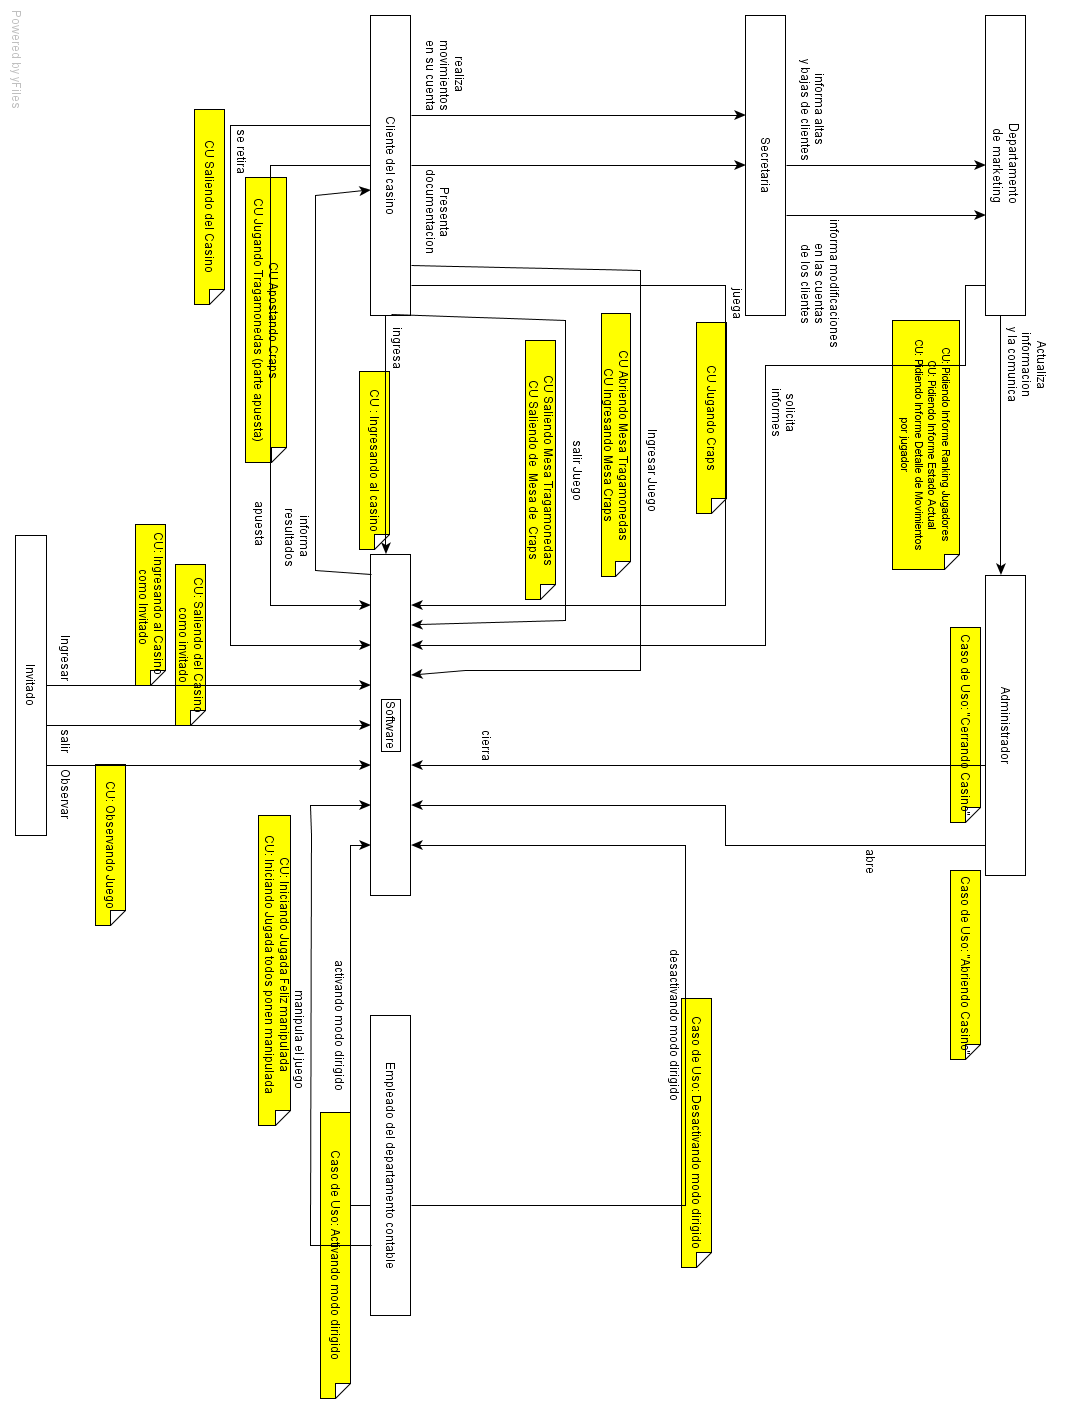
\includegraphics[scale=0.38]{img/dcCasino.png}
\end{center}

\begin{framed}

\depto Todas las interacciones de los agentes con el sistema han sido asignadas a uno o mas Casos de Uso que explicaran de forma mas detallada dichas interacciones. De esta manera podemos garantizar que las interacciones mas relevantes del sistema seran correctamente detalladas

\end{framed}

\subsection{Interacciones de agentes externos con el sistema}

{\large Casos de Uso \label{fig:cuCasino}}
\begin{center}
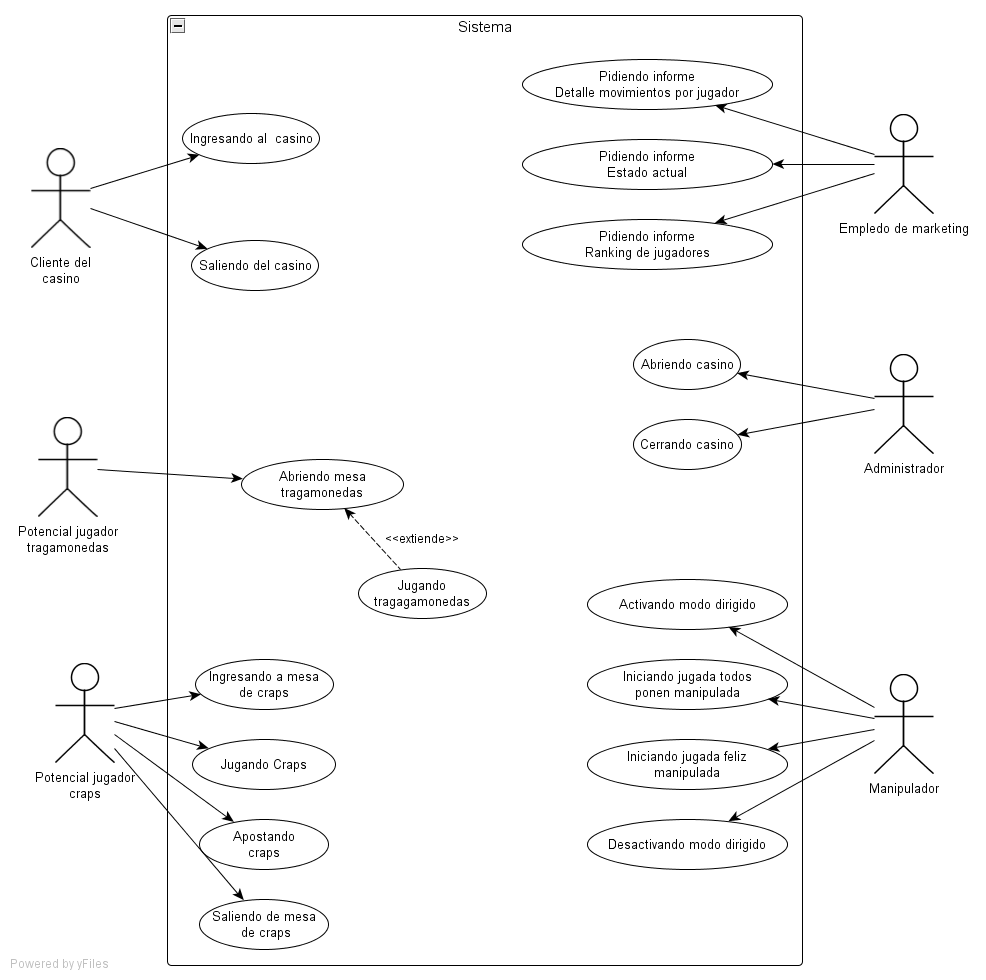
\includegraphics[scale=0.38]{img/casosDeUso.png}
\end{center}

{\large Casos de Uso - Herencia \label{fig:herencia}}
\begin{center}
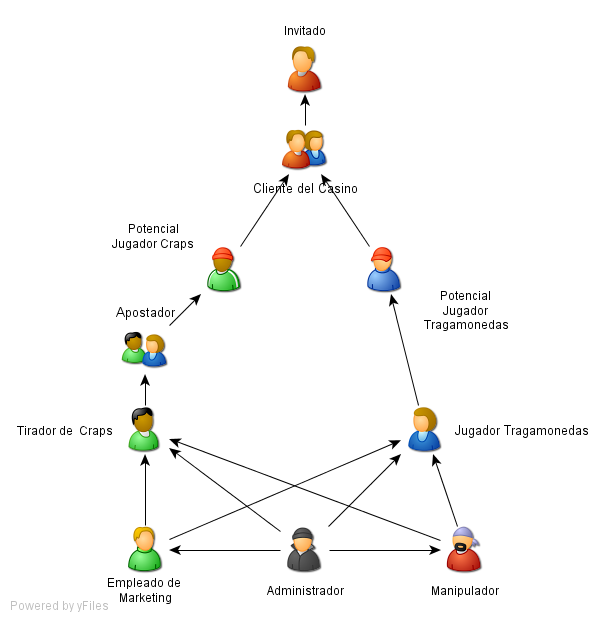
\includegraphics[scale=0.38]{img/herencia.png}
\end{center}

%%%%%%%ACTORES
%%%%%%\newcommand{\pc}{{\bf Cliente del casino }}
%%%%%%\newcommand{\adm}{{\bf Administrador }}
%%%%%%%\newcommand{\ptra}{{\bf Potencial jugador de tragamonedas }}
%%%%%%\newcommand{\jutra}{{\bf Jugador de Tragamonedas }}
%%%%%%\newcommand{\jc}{{\bf Jugador de Craps }}
%%%%%%\newcommand{\jac}{{\bf Apostador de Craps }}
%%%%%%\newcommand{\emc}{{\bf Empleado Contable }}
%%%%%%\newcommand{\emk}{{\bf Empleado de Marketing }}
%%%%%%\newcommand{\aptra}{{\bf Apostador de Tragamonedas }}
%%%%%%\newcommand{\apocr}{{\bf Apostador de Craps }}
%%%%%%\newcommand{\jucr}{{\bf Potencial Jugador de Craps }}
%%%%%%%CASOS DE USO
%%%%%%\newcommand{\ic}{{\bf Ingresando a casino }}
%%%%%%\newcommand{\salc}{{\bf Saliendo del casino }}
%%%%%%\newcommand{\atra}{{\bf Abriendo Mesa Tragamonedas }}
%%%%%%\newcommand{\jtra}{{\bf Jugando Tragamonedas }}
%%%%%%\newcommand{\actm}{{\bf Activando Modo Dirigido }}
%%%%%%\newcommand{\desm}{{\bf Desactivando Modo Dirigido }}
%%%%%%\newcommand{\jugf}{{\bf Jugada Feliz }}
%%%%%%\newcommand{\jugtp}{{\bf Jugada Todos Ponen }}
%%%%%%\newcommand{\ac}{{\bf Abriendo Casino }}
%%%%%%\newcommand{\cc}{{\bf Cerando Casino }}
%%%%%%\newcommand{\apotra}{{\bf Apostando en Tragamonedas }}
%%%%%%\newcommand{\incr}{{\bf Ingresando a mesa de Craps }}
%%%%%%\newcommand{\scr}{{\bf Saliendo de mesa de Craps }}
%%%%%%\newcommand{\jcr}{{\bf Jugando Craps }}
%%%%%%\newcommand{\apcr}{{\bf Apostando Craps }}
%%%%%%\newcommand{\admin}{{\bf administrador}}
%%%%%%\newcommand{\ccas}{{\bf Cerrando Casino}}
%%%%%%\newcommand{\empmark}{{\bf Empleado de Marketing}}
%%%%%%\newcommand{\infomovjug}{{\bf Pidiendo informes}}
%%%%%%\newcommand{\infoestact}{{\bf informe Estado Actual}}
%%%%%%\newcommand{\inforankjug}{{\bf informe Ranking de Jugadores}}
%%%%%%\newcommand{\infdmj}{{\bf Pidiendo informe Detalles de movimientos por jugador}}
%%%%%%\newcommand{\infea}{{\bf Pidiendo informe Estado Actual}}
%%%%%%\newcommand{\infrj}{{\bf Pidiendo informe Ranking de Jugadores}}


\newcommand{\req}{{\bf Requerimientos satisfechos por este Caso de Uso: }}
%ACTORES
\newcommand{\pc}{{\bf Cliente del casino }}
\newcommand{\adm}{{\bf Administrador }}
\newcommand{\invi}{{\bf Invitado }}
%\newcommand{\ptra}{{\bf Potencial jugador de tragamonedas }}
\newcommand{\jutra}{{\bf Jugador de Tragamonedas }}
\newcommand{\pjc}{{\bf Potencial jugador de Craps }}
\newcommand{\jc}{{\bf Jugador de Craps }}
\newcommand{\apcr}{{\bf Apostador de Craps }}
\newcommand{\emc}{{\bf Empleado Contable }}
\newcommand{\emk}{{\bf Empleado de Marketing }}
\newcommand{\jucr}{{\bf Tirador de Craps}}
\newcommand{\mani}{{\bf Manipulador }}
%CASOS DE USO
\newcommand{\ic}{{\bf Ingresando al casino }}
\newcommand{\salc}{{\bf Saliendo del casino }}
\newcommand{\inginvi}{{\bf Ingresando al casino como invitado}}
\newcommand{\salinvi}{{\bf Saliendo del casino como invitado }}
\newcommand{\obser}{{\bf Observando Juego }}
\newcommand{\intr}{{\bf Ingresando a mesa de Tragamonedas }}
\newcommand{\jtra}{{\bf Jugando Tragamonedas }}
\newcommand{\satr}{{\bf Saliendo a mesa de Tragamonedas }}
\newcommand{\incr}{{\bf Ingresando a mesa de Craps }}
\newcommand{\jugcr}{{\bf Jugando Craps }}
\newcommand{\apocr}{{\bf Apostando Craps }}
\newcommand{\sacr}{{\bf Saliendo a mesa de Craps }}
\newcommand{\actm}{{\bf Activando Modo Dirigido }}
\newcommand{\desm}{{\bf Desactivando Modo Dirigido }}
\newcommand{\jugf}{{\bf Iniciando Jugada Feliz Manipulada}}
\newcommand{\jugtp}{{\bf Iniciando Jugada Todos Ponen Manipulada}}
\newcommand{\ac}{{\bf Abriendo Casino }}
\newcommand{\cc}{{\bf Cerrando Casino }}
\newcommand{\infdmj}{{\bf Pidiendo informe Detalles de movimientos por jugador}}
\newcommand{\infea}{{\bf Pidiendo informe Estado Actual}}
\newcommand{\infrj}{{\bf Pidiendo informe Ranking de Jugadores}}

\subsection{Conceptos fundamentales, y sus relaciones}

\subsubsection{Conceptos fundamentales}
Identificamos y explicamos los conceptos funadamentales y las propiedades definitorias de ellos, y los estructuramos en un Modelo Conceptual\footnote{Casa caja representa una agrupacion de objetos reconocidos del dominio del problema que se caracterizan por tener propiedades similares, las lineas son asociaciones estre estos conceptos que indica alguna vinculacion significativa entre ellos}.\\
Explicamos brevemente que representa cada uno de estos conceptos.

\begin{itemize}

	\item Jornada: Contiene la informacion general del casino

	\item ResultadoPosibleCraps: Representa todas los resultados a una jugada, que finalizan una apuesta particular. (representa a la accion concreta de perder o ganar para una apuesta, los resultados que no definen la apuesta, no aparecen)

	\item Jugador: Repesenta a un jugador del casino.

	\item MesaTragamonedas: repesenta todas las mesas de tragamonedas que se abrieron desde que se abrio el casino (Cada mesa que es o fue usada por un jugadr del casino). Dicha mesa no se reabre.

	\item ResutadoPosibleTragamonedas: Representa todas los resultados a una jugada, que finalizan una apuesta particular. (representa a la accion concreta de perder o ganar para una apuesta, los resultados que no definen la apuesta, no aparecen)

	\item JugadaTragamonedas: Repesenta al conjunto de jugadas de todas las mesas de tragamonedas.

	\item ApuestaTragamonedas: Repesenta al conjunto de las asociacion entre una jugada de tragamonedas y el jugador que esta jugando (En el tragamonedas es imposible jugar sin apostar, y cada jugada teniene asociada una apuesta articular).

	\item TipoDeJugada: Repesta el tipo de jugada que esta asociado a toda jugada del casino, tanto sea de craps como tragamonedas.

	\item JugadaFeliz: Representan al tipo de jugada que tiene asociado el pago del premio ``Pozo Feliz''.

	\item JugadaTodosPonen: Representa al tipo de jugada que tiene asociado el cobre de porcentajes para el incremento del pozo feliz.

	\item JugadaNormal: Repesenta al tipo de jugada normal, es decir una jugada con el comportamiento comun.

	\item ApuestasCraps: Representa todas las apuestas que se hacen en cada jugada de cada mesa de craps.

	\item MesaCraps: repesenta todas las mesas de craps que se abrieron desde que se abrio el casino (Cada mesa que es o fue usada por un jugadr del casino). Dicha mesa no se reabre.

	\item JugadaCraps: Representa cada uno de los tiros de dados que se hacen en ua mesa de craps.

\end{itemize}

\subsubsection{Modelo Conceptual}

\begin{center}
		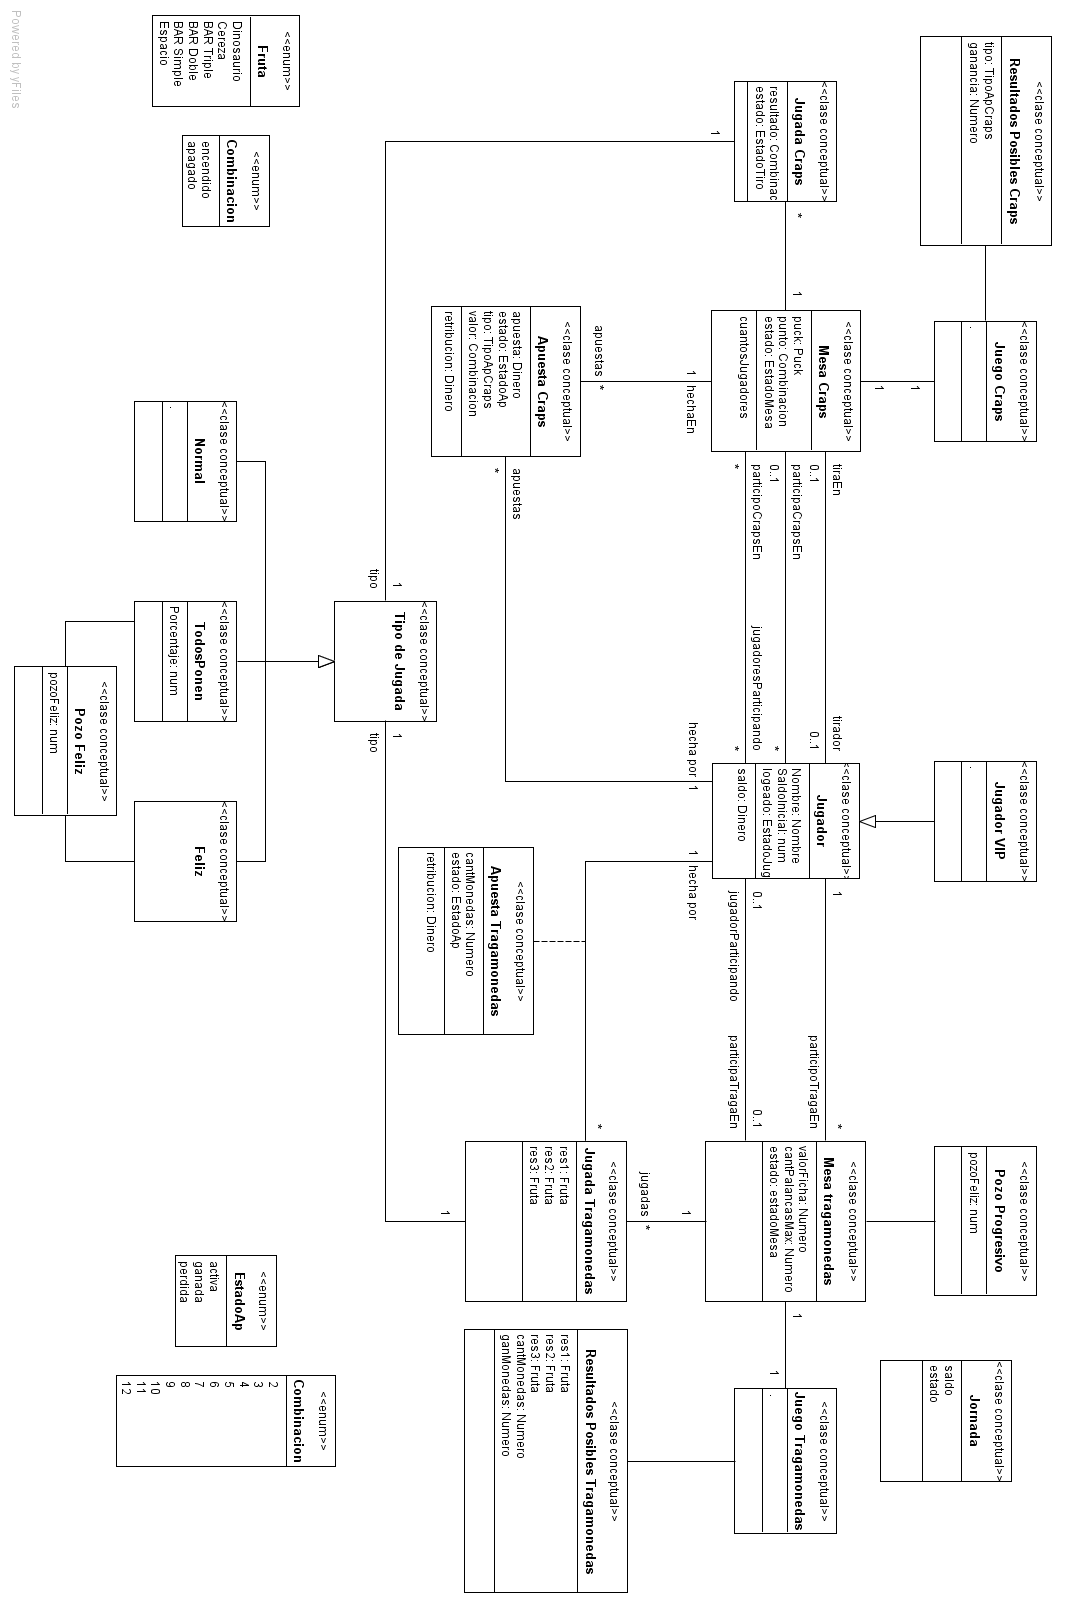
\includegraphics[scale=0.45]{img/dclCasino.png}
\end{center}

Dado las limitaciones del Modelo Conceptual, agregaremos algunos invarientes para identificar mejor los estados deseables del sistema. 


\begin{framed}
\depto Dado las limitaciones del Modelo Conceptual, agregaremos algunos invarientes para identificar mejor los estados deseables del sistema.

\subsection{Invariantes relacionados con el estado general del sistema}
\lstset{language=ocl}
\lstset{commentstyle=\textit}
\begin{lstlisting}[frame=trbl]{}

-----------------------
-- POZOS
-----------------------
-- hay un unico pozo progresivo
context PozoProgresivo
inv UnicoPozoProgresivo:
PozoProgresivo.allInstances()->size() = 1

-- hay un unico pozo feliz
context PozoFeliz
inv PozoFeliz:
PozoFeliz.allInstances()->size() = 1

-- el monto del pozo progresivo es mayor a 0
context PozoProgresivo
inv PozoProgresivoNoNegativo:
PozoProgresivo.allInstances()->asSecuence().first().monto > 0

-- el monto del pozo feliz es mayor a 0
context PozoFeliz
inv PozoFelizNoNegativo:
PozoFeliz.allInstances()->asSecuence().first().monto > 0

-----------------------
-- RESULTADOS POSIBLES
-----------------------
-- hay como maximo un resultado posible por cada combinacion 
-- del juego tragamonedas
context ResultadoPosibleTragamonedas
inv UnResultadoPorPremioTraga:
ResultadoPosibleTragamonedas.allInstances()->
   forAll(r | r <> self -> r.res1 <> self.res1 or
                           r.res2 <> self.res2 or
                           r.res3 <> self.res3 )

-- hay como maximo un resultado posible por cada combinacion 
-- del juego craps
context ResultadoPosibleCraps
inv UnResultadoPorPremioCraps:
ResultadoPosibleCraps.allInstances()->
   forAll(r | r <> self -> r.tipo <> self.tipo or
                           r.numero.oclIsUndefined() or
   not(r.numero.oclIsUndefined()) implies r.numero <> self.numero or
                           r.res3 <> self.res3 )

-----------------------
-- JUGADOR
-----------------------

-- un jugador comun no puede tener saldo 
-- negativo a menos que sea VIP
context Jugador
inv JugadorComunNoPuedePoseerSaldoNegativo:
not(self.oclInstanceOf(JugadorVIP)) implies self.saldo >= 0

-- un jugador no puede participar en mas de un juego
cantext Jugador
inv NoParticiparEnMasDeUnJuego:
not(self.participaCrapsEn.oclIsUndefined()) implies 
   self.participaTragaEn.oclIsUndefined() and
not(self.participaTragaEn.oclIsUndefined()) 
   implies self.participaCrapsEn.oclIsUndefined()

-- un jugador no logeado no puede estar participando de un juego
context Jugador
inv NoLogeadoEntoncesNoJugando
self.estado = EstadoJugador::NoLogeado implies 
  ( self.participaTragaEn.oclIsUndefined() and 
    self.participaCrapsEn.oclIsUndefined() )

-- un jugador no puede participar en una mesa cerrada
cantext Jugador
inv NoParticiparEnMesaCerrada:
not(self.participaCrapsEn.oclIsUndefined()) implies 
   self.participaTragaEn.estado = EstadoMesa:Abierta and
not(self.participaTragaEn.oclIsUndefined()) 
   implies self.participaCrapsEn.estado = EstadoMesa:Abierta
   
\end{lstlisting}


\subsection{Invariantes relacionados con el juego tragamonedas}
\lstset{language=ocl}
\lstset{commentstyle=\textit}
\begin{lstlisting}[frame=trbl]{}

--Si un jugador tiene apuestas activas de tragamonedas,
--esta participando de una mesa de tragamonedas
context Jugador
inv ApuestasActivasEntoncesParticipaEnMesa:
self.ApuestasTragamonedas->exists(a | a.estado = EstadoAp::Activa)
    implies not(self.participaTragaEn.oclIsUndefined())

--Si un jugador esta participando de una mesa, 
--dicha mesa debe estar abierta
context Jugador
inv ParticipandoEnMesaEntoncesMesaActiva:
not(self.participaTragaEn.oclIsUndefined()) implies
    self.participaTragaEn.estado = EstadoMesa::Abierta

--si una mesa esta abierta tiene un jugador participando 
--y si esta cerrada no debe poseer ningun jugador participando
context MesaTragamonedas
inv AbiertaTragaEntoncesJugadorParticipando:
(self.estadoMesa = EstadoMesa::Abierta) implies 
    not(self.jugadorParticipando.oclIsUndefined()) and
(self.estadoMesa = EstadoMesa::Cerrada) implies 
    self.jugadorParticipando.oclIsUndefined()

--las apuestas activas de un jugador deben estar relacionadas 
--con la mesa en la que esta jugando dicho jugador
context Jugador
inv ApuestasActivasEnMesaEnLaQueEstoyJugando:
self.ApuestasTragamonedas->
    forAll(a | a.estado = EstadoAp::Activa implies 
    a.JugadaTragamonedas.mesaTragamonedas = self.participaTragaEn)

--si una mesa esta cerrada no debe poseer ninguna apuesta activa
context MesaTragamonedas
inv MesaTragaCerradaSinApuestasActivas:
(self.estado = EstadoMesa::Cerrada) implies 
((self.jugadaTragamonedas->
    forAll(j | j.apuestaTragamonedas.estado = EstadoAp::Ganada or 
               j.apuestaTragamonedas.estado = EstadoAp::Perdida)

--todas las apuestas de un jugador corresponden a 
--una mesa en la que participo
context Jugador
self.apuestasTragamonedas->forAll(a | self.participoEn->
    includes(a.jugadaTragamonedas.mesa) )
\end{lstlisting}

\subsection{Invariantes relacionados con el juego craps}

\lstset{language=ocl}
\lstset{commentstyle=\textit}
\begin{lstlisting}[frame=trbl]{}
-- Si un jugador tiene apuestas activas de craps,
-- esta participando de una mesa de craps
context Jugador
inv ApuestasActivasCrapsEntoncesParticipaEnMesaCraps:
self.ApuestasCraps->exists(a | a.estado = EstadoAp::Activa)
    implies not(self.participaCrapsEn.oclIsUndefined())
    
    
--Si un jugador esta participando de una mesa, 
--dicha mesa debe estar abierta
context Jugador
inv ParticipandoEnMesaCrapsEntoncesMesaActiva:
not(self.participaTragaEn.oclIsUndefined()) implies
    self.participaTragaEn.estado = EstadoMesa::Abierta

-- si una mesa esta abierta tiene un jugador 
-- participando y un jugador tirando
--
-- y si esta cerrada no debe poseer ningun jugador 
-- participando ni tirando
context MesaCraps
inv AbiertaCrapsEntoncesJugadorParticipando:
(self.estadoMesa = EstadoMesa::Abierta) implies 
    (not(self.jugadorParticipando.oclIsUndefined()) and
    not(self.tirador.oclIsUndefined())) and
(self.estadoMesa = EstadoMesa::Cerrada) implies 
    (self.jugadorParticipando.oclIsUndefined() and
    self.tirador.oclIsUndefined())
    
--las apuestas activas de un jugador deben estar relacionadas 
--con la mesa en la que esta jugando dicho jugador
context Jugador
inv ApuestasActivasCrapsEnMesaEnLaQueEstoyJugando:
self.apuestasCraps->
    forAll(a | a.estado = EstadoAp::Activa implies 
self.participaCrapsEn ->including(a.hechaEn.mesaCraps)

--si una mesa esta cerrada no debe poseer ninguna apuesta activa
context MesaCraps
inv MesaCrapsCerradaSinApuestasActivas:
(self.estado = EstadoMesa::Cerrada) implies 
((self.apuestaCraps->
    forAll(a | a.estado = EstadoAp::Ganada or 
               a.estado = EstadoAp::Perdida)

--todas las apuestas de un jugador corresponden a 
--una mesa en la que participo
context Jugador
self.apuestasCraps->forAll(a | self.participoEn->
    includes(a.hechaEn) )

Queries:

Query

context: Mesa Craps::CuantosJugadores : numero
body: self.Jugador.allInstances->select(x 
					| x.participaCrapsEn = self)->sum() 



\end{lstlisting}
\end{framed}



\subsection{Lista de Requerimientos}

\newcommand{\ii}{{\bf Importante }}
\newcommand{\ff}{{\bf Funcional }}
\newcommand{\dd}{{\bf Deseable }}
\newcommand{\nd}{{\bf No deseable }}
\newcommand{\nf}{{\bf No funcional }}
\newcommand{\ee}{{\bf Esencial }}

\newcommand{\rrr}{{ \\ \bf REFERIDO EN: }}

\begin{enumerate}

\item\textsc{REQUERIMIENTOS GENERALES DEL CASINO - MANEJO DE CLIENTES}
\begin{enumerate}
\item Los clientes no podr�n apostar mas que el saldo permitido por el departamento de marketing: Los clientes tendr�n un saldo limite y no podr�n realizar ningun tipo de apuesta que sobrepase ese saldo.  \ff - \ii. \rrr \ref{1a1} y en \ref{1a2}
\item Los clientes VIP podr�n apostar ilimitadamente: Los clientes VIP no tiene limite de saldo, por lo tanto no habra ningun monto de apuesta que pueda ser invalidado.  \ff - \ii. \rrr \ref{1b1} y en \ref{1b2}
\item VER Un invitado podr� observar los juegos pero sin participar en ellos: Puede ingresar en una mesa ya abierta y observar el desarrollo del juego pero sin intervenir en el. \ff - \dd. \rrr \ref{1c}
\item Se deber� modificar el saldo del cliente en cada apuesta: Cada vez que un cliente haga una apuesta de cualquier tipo se vera reflejado en la disminuci�n de su saldo.  \ff - \ii. \rrr \ref{1d1} y en \ref{1d2}
\end{enumerate}

\item\textsc{REQUERIMIENTOS GENERALES DEL CASINO - MANEJO DE MESAS}
\begin{enumerate}
\item No se debe permitir que un jugador juegue en mas de una mesa al mismo tiempo: Para ingresar a una mesa de cualquier juego el jugador no podr� estar adentro de ninguna otra mesa de ningun juego.  \ff - \dd. \rrr \ref{2a1} y en \ref{2a2}
\item Los clientes podr�n abrir mesas: Todos los clientes tendran la opci�n de abrir una nueva mesa para cualquiera de los juegos.  \ff - \ee
\item Los clientes podr�n unirse a mesas (s� el juego lo permite): El tragamonedas no permite unirse a una mesa, pero en el Craps el jugador podr� elegir a cual de las mesas habilitadas se unir�.  \ff - \ii
\item Las mesas vacias se cerraran autom�ticamente: Cuando un jugador salga de un juego el sitema autom�ticamente cerrara la mesa a menos que haya otros jugadores en ella.  \ff - \ee
\item El casino no se podr� cerrar mientras haya gente jugando: El casino solo podr� cerrar cuando todos los jugadores hayan salido del mismo.  \ff - \ii
\item No debe haber limite de mesas abiertas: Los clientes podr�n ingresar a las mesas de los juegos y no habra un limite de ellas.  \ff - \ii
\end{enumerate}

\item\textsc{REQUERIMIENTOS GENERALES DEL CASINO - PANTALLA}
\begin{enumerate}
\item Las pantallas mostraran la informaci�n necesaria para el desarrollo del juego: Las pantallas mostrar�n la interfaz del juego asi como tambien todas las opciones disponibles dentro del juego.  \ff - \ii
\item Las pantallas mostraran la informaci�n necesaria del estado del juego: Las pantallas mostraran el tipo de jugada, estado actual del juego y resultados, y ser� inmediatamente actualizada ante cualquier cambio o variaci�n.  \ff - \ii
\item Las pantallas mostraran el estado de la cuenta del jugador: Por pantalla se podr� ver si un jugador esta dentro del casino y dentro de algun juego y si es as� en que mesa, si ha resultado ganador o no, y su correspondiente saldo.  \ff - \dd
\end{enumerate}

\item\textsc{REQUERIMIENTOS GENERALES DEL CASINO - CONFIGURACION}
\begin{enumerate}
\item Permitir la configuraci�n est�tica del monto m�nimo de los pozos: Se podr� permitir configurar el monto minimo que debe superar un pozo antes de poder entregarlo.  \nf - \dd
\end{enumerate}

\item\textsc{REQUERIMIENTOS GENERALES DEL CASINO - FICHAS}
\begin{enumerate}
\item Las apuestas se har�n por medio de fichas: En todos los juegos el jugador podr� elegir el monto a apostar seleccionando de entre los valores establecidos de las fichas.  \ff - \ii
\item Las fichas ser�n ilimitadas: No habra una cantidad fija de fichas sino que se dispondr� de ellas en un numero ilimitado.  \ff - \ii
\item El valor de las fichas debe poder configurarse por el administrador: Cada vez que el casino abre al administrador configurara los valores posibles de las fichas.  \nf - \ii
\end{enumerate}

\item\textsc{REQUERIMIENTOS GENERALES DEL CASINO - REPORTES}
\begin{enumerate}
\item Generar informe electr�nico: Ranking de jugadores: Se generar� un informe con los jugadores que m�s dinero ganaron en el d�a desde que abrio el casino, como tambi�n los que m�s dinero perdieron. \ff - \ii
\item Generar informe electronico: Estado Actual: Se generar� un informe con el estado del casino y su saldo y tambi�n el de los clientes. \ff - \ii
\item Generar informe electronico: Detalle de movimientos por jugador: Se generar� un informe con todas las apuestas, premios ganados, y montos ganados por cada jugador que haya ingresado al casino. \ff - \ii
\end{enumerate}

\item\textsc{REQUERIMIENTOS GENERALES DEL CASINO - JUGADAS Y POZOS}
\begin{enumerate}
\item Mostrar en todo momento el monto de los pozos: En todo momento se mostrara el monto actualizado de todos los pozos del casino, y se actualizar� inmediatamente a medida que varie. \ff - \ii
\item Generar jugada feliz autom�ticamente: La jugada feliz se generara en base a probabilidades.  \ff - \ee
\item Generar jugada todos ponen autom�ticamente: La jugada todos ponen tambien se generara en base a probabilidades.  \ff - \ee
\item No se debe permitir el solapamiento de jugadas felices en el mismo instante: Si ha ocurrido una, entonces no podra ocurrir otra hasta que se pague la jugada existente y se supere el monto minimo, aunque pueden ocurrir en cualquiera de las mesas del casino pero no simultaneamente.  \ff - \ii
\end{enumerate}

\item\textsc{REQUERIMIENTOS GENERALES DEL CASINO - MODO DIRIGIDO}
\begin{enumerate}
\item El sistema deber� contar con un modo dirigido: Se podra poner en modo dirigido a cada uno de los juegos y todas sus respectivas mesas tendr�n como resultado el definido por el manipulador de modos.  \ff - \ii
\item El sistema deber� permitir generar jugada feliz manualmente: El manipulador de modos podr� decidir la ocurrencia de jugadas felices mientras no se solapen simultaneamente en los juegos del casino.  \ff - \ii
\item El sistema deber� permitir generar jugada todos ponen manualmente: El manipulador de modos podr� decidir la ocurrencia de jugadas todos ponen mientras no se solapen en la misma jugada. \ff - \ii
\end{enumerate}

\item\textsc{REQUERIMIENTOS DE JUEGO TRAGAMONEDAS}
\begin{enumerate}
\item Proveer juego Tragamonedas: Se proveera el juego del Tragamonedas respetando las reglas provistas por los clientes.  \ff - \ee. \rrr \ref{9a}
\item El juego Tragamonedas debe contar con un premio gordo progresivo: El juego de Tragamonedas permitira incrementar el premio gordo progresivo usando un porcentaje de cada una de las jugadas para ser otorgado luego de superar el monto minimo configurado al que obtenga la combinacion ganadora y haya apostado las n veces anteriores al maximo numero de fichas. \ff - \ee. \rrr \ref{9b}
\item El cliente podr� elegir entre varios valores de fichas de las maquinas tragamonedas: Se podr� elegir una mesa de maquina tragamonedas de distintos valores entre los definidos. Una vez elegido el valor de la ficha para el tragamonedas este no se podr� cambiar hasta salir del juego.  \ff - \nd. \rrr \ref{9c}
\end{enumerate}

\item\textsc{REQUERIMIENTOS DE JUEGO CRAPS}
\begin{enumerate}
\item Proveer juego Craps: Se proveera el juego de Craps respetando las reglas provistas por los clientes. \ff - \ee. \rrr \ref{10a}
\end{enumerate}

\item\textsc{REQUERIMIENTOS DE IMPLEMENTACION Y COMPORTAMIENTO}
\begin{enumerate}
\item El sistema debe funcionar en red.  \nf - \ee
\item VER El sistema a implementarse deber� estar realizado en Java o C$\#$ \nf - \ii 
\item VER El sistema debe ser facilmente extendible con nuevos juegos \nf - \ii 
\end{enumerate}


\item\textsc{REQUERIMIENTOS DE FUNCIONALIDAD EXTRA}
\begin{enumerate}
\item VER Se podr�n ver imagenes de los juegos en 3D \ff - \dd
\item VER Los jugadores podran chatear entre ellos dentro del juego \ff - \dd
\end{enumerate}

\end{enumerate}




\subsection{Registracion y Ingreso al casino online y modificacion de saldo}

\subsubsection{Registracion}
Segun lo acordado, la registracion de los usuarios se hace por fuera del sistema informatico del casino online. Explicaremos como esperamos que interactuen los agentes externos para que el sistema posea la lista actualizada de usuarios registrados. Para ello usaremos el Diagrama de Activdades\footnote{Diagrama de Actividades: Grafico que representa el flujo de actividades. Las cajas representan actividades y las flechas repersentan secuencialidad y los rombos representan decisiones} ``Registracion''. Ver Figura: \ref{fig:daReg}

{\large Diagrama de actividades Registracion\label{fig:daReg}}
\begin{center}
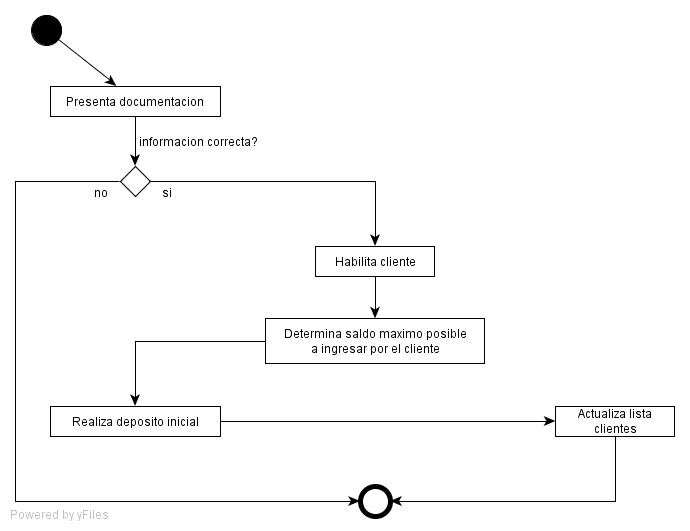
\includegraphics[scale=0.5]{img/daRegistracion.png}
\end{center}

Cabe aclarar que el cliente podra comenzar a jugar en el casino recien cuando el casino se vuelva a abrir

\subsubsection{Modificacion de saldo}

Una vez registrado un cliente puede ingresar y retirar dinero real, dicha operacion solo podra realizarse mistras el casino permanece cerrado.
Explicaremos esta operatoria con un diagrama de actividades. Ver Figura: \ref{fig:modSaldo}

{\large Diagrama de actividades Modificacion de Saldo\label{fig:modSaldo}}
\begin{center}
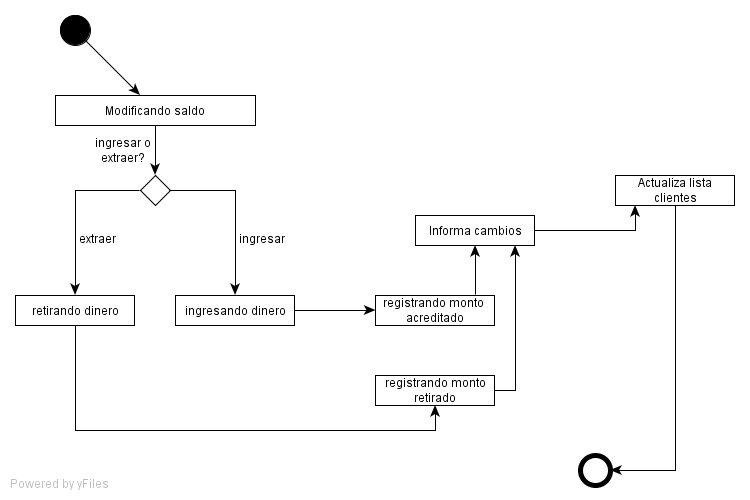
\includegraphics[scale=0.4]{img/clienteModSaldo.png}
\end{center}

\subsubsection{Ingreso y egreso del casino}

La forma en que un cliente ingresa o egresa del casino esta explicado en los casos de uso: \\
CU \ic \ref{lic} y CU \salc \ref{lsalc}.

%----------------------------------------------------------
% CASO DE USO INGRESANDO A CASINO
%----------------------------------------------------------
\label{lic}

\begin{cu}{\ic}
	\descripxizq=1cm
		\defln{Este caso de uso explica como un \pc ingresa en el casino }
		\actor{\pc}
		\pre{El casino debe estar abierto y el jugador debe estar fuera del casino}
		\post{El \pc ha ingresado al casino }

	\begin{cursoe}{}
	
		\paso{1 El \pc ingresa su nombre de usuario}{}
		
		\paso{2 El sistema verifica si el nombre corresponde a un usuario valido}{}
		
		\paso{3 El sistema ingresa al \pc al casino}{}
		
		\paso{4 El sistema informa que el \pc ha ingresado al casino satisfactoriamente}{4.1 El sistema informa que el usuario es invalido. Ir a paso 5}
		
		\paso{5 Fin C.U.}{}	
		
	\end{cursoe}
	
\end{cu}

%----------------------------------------------------------
% CASO DE USO SALIENDO DEL CASINO
%----------------------------------------------------------
\label{lsalc}

\begin{cu}{\salc}
	\descripxizq=1cm
		\defln{Este caso de uso explica como un \pc sale del casino }
		\actor{\pc}
		\pre{El casino debe estar abierto y el \pc debe estar dentro del casino}
		\post{El \pc ha salido del casino }

	\begin{cursoe}{}
		
		\paso{1 Si el \pc no esta jugando ir a paso 4}{}
		
		\paso{2 El sistema informa que de continuar, perder� todas las apuestas activas}{}
	
		\paso{3 El sistema cancela todas las apuestas del \pc, y lo retira de la mesa correspondiente}{3.1 El \pc cancela la operacion ir a paso 6}
		
		\paso{4 El sistema retira al \pc del casino}{}
		
		\paso{5 El sistema informa que el \pc ha salido del casino}{}
		
		\paso{6 Fin C.U.}{}
		
	\end{cursoe}
	
\end{cu}


\subsection{Administracion del Casino}

\subsubsection{Apertura del casino}

El administrador puede realizar configuraciones de distintos aspectos:
\begin{itemize}
	\item Configuracion de valores de fichas
	\item Asignacion de probablilidades
	\item valores minimos para la entrega de premios
\end{itemize}
Al realizarse la apertura del casino, el sistema carga automaticamente un archivo donde se encuentran establecidas las configuracion efectuadas por el administrador. 

\begin{center}
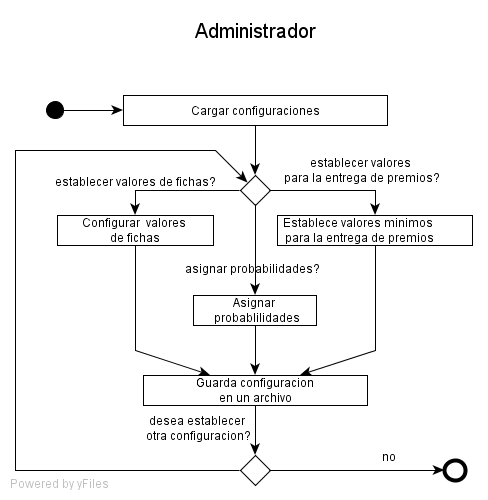
\includegraphics[scale=0.38]{img/configuraciones.png}
\end{center}

Con el caso de uso CU \ac \ref{lac} explicaremos la interaccion con el sistema. 

%----------------------------------------------------------
% CASO DE USO ABRIENDO CASINO
%----------------------------------------------------------
\label{lac}

	\begin{cu}{\ac}
	\descripxizq=1cm
		\defln{ Este caso de uso explica como se abre el casino }
		\actor{\admin}
		\pre{ El casino debe estar cerrado }
		\post{ El casino esta abierto}

	\begin{cursoe}{}
	
		\paso{1 El \admin ingresa al sistema la lista actualizada de los clientes }{}
		\paso{2 El \admin configura los valores de las fichas que se usaran en la jornada}{}
		\paso{3 El \admin configura el porcentaje de la jugada todos ponen }{}
		\paso{4 El \admin determina los valores minimos para la entrega de premios}{}
		\paso{5 El sistema informado que se ha iniciado un nuevo dia}{}
		
		\paso{ Fin C.U.}{}
		

	\end{cursoe}
\end{cu}

\subsubsection{Clausura del casino}

La operatioria de cerrar el casino no es muy complicada, pero tiene una salvedad. No es posible cerrar el casino si hay jugadores dentro del casino

Dicha interaccion con el sistema esta explicada en el caso de uso: CU \ccas \ref{lccas}

%----------------------------------------------------------
% CASO DE USO CERRANDO CASINO
%----------------------------------------------------------

\label{lccas}

\begin{cu}{\ccas}
	\descripxizq=1cm
		\defln{ Este caso de uso explica como se cierra el casino }
		\actor{\admin}
		\pre{ El casino debe estar abierto }
		\post{ El casino esta cerrado}

\begin{cursoe}{}
	
		\paso{1 El \admin cierra el casino }{}
		\pasoa{2 El sistema informa que el casino se cerrara}{2.1 El sistema notifica que hay mesas abiertas. No se puede 							cerrar. Ir a paso 3}
		\paso{ Fin C.U.}{}
		

	\end{cursoe}
\end{cu}

\begin{framed}

\depto Con esta maquina de estados finitos (FSM) Mostramos que nos comprometemos a que un administrador podr� cerrar el casino solo si no hay ningun cliente en el mismo.

{\large FSM: Administrador}
\begin{center}
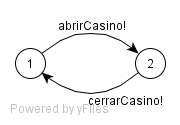
\includegraphics[scale=0.5]{img/admin.png}
\end{center}


{\large FSM: Jugador$_i$}
\begin{center}
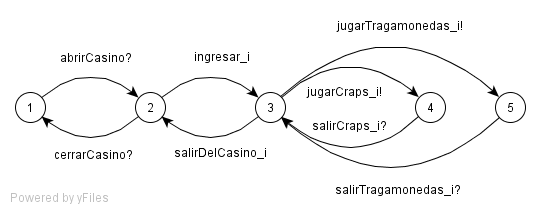
\includegraphics[scale=0.5]{img/jugador.png}
\end{center}

\textbf{Nota}: la interaccion que tiene un jugador con cada uno de los juegos se puede observar en los apartados `JUEGO TRAGAMONEDAS' y `JUEGO CRAPS'. 


\end{framed}

\subsection{Invitado}
El casino brinda una modalidad para entrar a los juegos como invitado. Bajo este modalidad aquella persona que ingrese al casino podra observar el desarrollo de los juegos pero sin participar
La interaccion que posee un \textbf{\textit{invitado}} se explica con los CU (\textit{faltan los cu})

En el siguiente Diagrama de actividades se puede observar lo que puede hacer un invitado dentro del casino.

\begin{center}
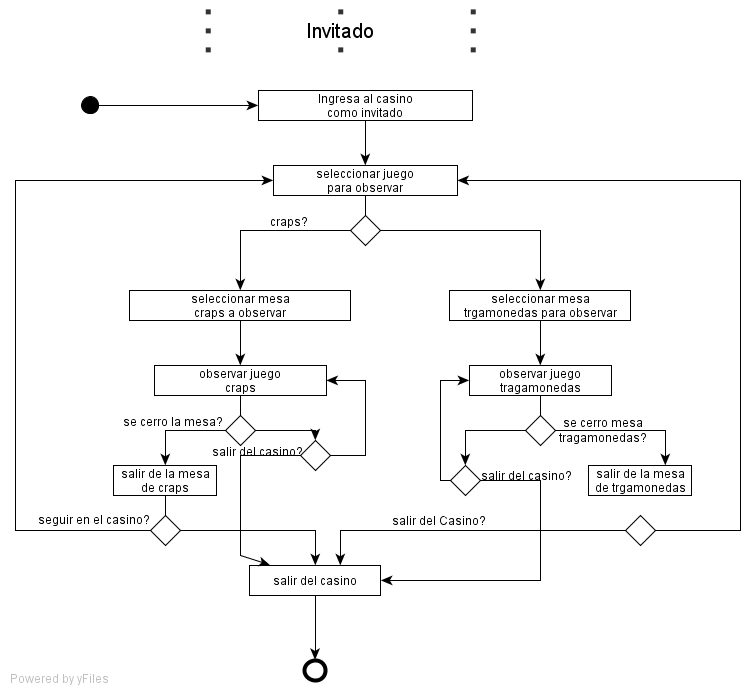
\includegraphics[scale=0.5]{img/invitado.png}
\end{center}





\subsection{Modo Dirigido}

\subsubsection{Inicio de Modo Dirigido}

Cuando se ingresa en este modo, los resultados de las jugadas no seran al azar sino que el manipulador decidira los mismos.

Esos resultados ingresados se respetaran para todas las jugadas de todas las mesas habilitadas de ese juego mientras no se vuelva a modo normal.

Dicha interaccion con el sistema esta explicada en el caso de uso: CU \actm \ref{lactm}

%----------------------------------------------------------
%CASO DE USO ACTIVANDO MODO DIRIGIDO
%----------------------------------------------------------
\label{lactm}
\begin{cu}{\actm}
	\descripxizq=1cm
		\defln{Este caso de uso explica como un manipulador puede activar el modo dirigido del casino}
		\actor{\adm}
		\pre{ El casino debe estar abierto y desactivado el modo dirigido}
		\post{ Se ha activado el modo dirigido }

	\begin{cursoe}{}
	
		\paso{1 El manipulador selecciona activar el modo dirigido del casino }{}
		
		\paso{2 El sistema activa el modo dirigido, desactiva las jugadas azarosas}{}
						
		\paso{3 El sistema informa que se ha activado el modo dirigido del casino y solicita ingresar el resultado de las jugadas}{}
		
		\paso{4 El manipulador ingresa el resultado de las jugadas}{}
		
  	\paso{5 El sistema modifica la configuraci�n del casino}{}	
		
		\paso{6 El sistema informa que el casino se encuentra ahora en modo dirigido }{}

		\paso{7 Fin C.U.}{}
		
	\end{cursoe}
\paragraph{Comentario: }
\begin{flushleft}
Nota al Dpto de Sistemas: asumimos que el ingreso de los resultados de las jugadas es una configuraci�n dada
%me refiero a q ingresa un "archivo" con cierta configuracion ya armada para los result
\end{flushleft}
\end{cu}

\begin{framed}

\depto Con esta maquina de estados finitos (FSM) Mostramos que en modo dirigido se pueden lanzar jugadas de forma manual, dicha funcionalidad no esta permitida en modo normal.
Es seteo de las jugadas debe hacerse en el momento de entrar en modo dirigido. 

\paragraph{FSM: Manipulador}
\begin{center}
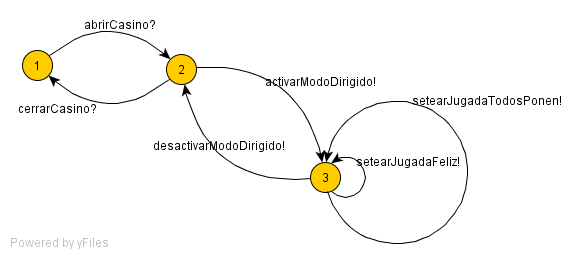
\includegraphics[scale=0.5]{img/manipulador.png}
\end{center}

\end{framed}

\subsubsection{Seteo de Jugadas Feliz y Todos Ponen}

El manipulador puede iniciar una Jugada Feliz, al hacerlo debe seleccionar una unica jugada que se ver� afectada por la Jugada Feliz.

Dicha interaccion con el sistema esta explicada en el caso de uso: CU \jugf \ref{ljugf}

%----------------------------------------------------------
%Caso de uso JUGADA FELIZ
%----------------------------------------------------------
\label{ljugf}
\begin{cu}{\jugf}
	\descripxizq=1cm
		\defln{ Este caso de uso explica como se seleccionara la aparici�n de las jugadas felices }
		\actor{\adm}
		\pre{ El casino est� abierto y esta activado el modo dirigido }
		\post{ Se ha generado una nueva aparicion de jugada feliz }

	\begin{cursoe}{}
	
		\paso{1 El \adm selecciona un juego }{}
		
		\paso{2 El \adm selecciona una jugada particular }{}
		
		\paso{3 El sistema genera una nueva jugada feliz }{3.1 ERROR El sistema informa que la jugada se solapa con otra jugada feliz en el mismo instante en el casino o con otra jugada todos ponen en el mismo juego y jugada}
	
		\paso{4 Fin C.U.}{}
		

	\end{cursoe}

\end{cu}

Por otro lado, si el manipulador inicia una Jugada Todos Ponen, al hacerlo puede seleccionar varias jugadas las cuales se veran afectadas (todas) por la jugada de este tipo.

Dicha interaccion con el sistema esta explicada en el caso de uso: CU \jugtp \ref{ljugtp}

%----------------------------------------------------------
%Caso de uso TODOS PONEN
%----------------------------------------------------------
\label{ljugtp}
\begin{cu}{\jugtp}
	\descripxizq=1cm
		\defln{ Este caso de uso explica como se seleccionara la aparici�n de las jugadas todos ponen }
		\actor{\adm}
		\pre{ El casino est� abierto y esta activado el modo dirigido }
		\post{ Se ha generado una nueva aparicion de jugada todos ponen }

	\begin{cursoe}{}
	
		\paso{1 El \adm selecciona un juego }{}
		
		\paso{2 El \adm selecciona las jugadas que se veran afectadas por la jugada todos ponen}{}
		
		\paso{3 El sistema genera una nueva jugada todos ponen }{}

		\paso{4 Fin C.U.}{}
		
	\end{cursoe}
\end{cu}	

\subsubsection{Finalizaci�n de Modo Dirigido}

En el momento que el manipulador decida abandoanar el modo dirigido, debera desactivarlo.
Y asi volver al modo normal. Ver caso de uso: CU \desm \ref{ldesm}

%----------------------------------------------------------
%Caso de uso Desactivando modo dirigido
%----------------------------------------------------------
\label{ldesm}
\begin{cu}{\desm}
	\descripxizq=1cm
		\defln{Este caso de uso explica como se desactiva el modo dirigido }
	  \actor{\adm}
		\pre{ El casino debe estar abierto y activado el modo dirigido }
		\post{ Se ha desactivado el modo dirigido y el resultado de las jugadas ser� aleatorio }
		
	\begin{cursoe}{}
	
		\paso{1 El manipulador selecciona desactivar el modo dirigido del casino}{}
		
		\paso{2 El sistema desactiva el modo dirigido activando los resultados azarosos para todas las jugadas y asi tambien las ocurrencias de los distintos tipos de jugadas }{}
		
		\paso{3 El sistema informa que el casino se encuentra ahora en modo normal }{}
		
		\paso{4 Fin C.U.}{}

	\end{cursoe}
	
\end{cu}
                                            
\subsection{Juego Tragamonedas}

Las m�quinas tragamonedas juegan con un �nico valor de ficha (Cuando se inicia el jugador elige dicho valor, entre los valores de fichas disponibles del casino). 

En el siguiente Diagrama de actividades se puede observar a grandes rasgos las actividades que realiza un jugador de tragamonedas.

\begin{center}
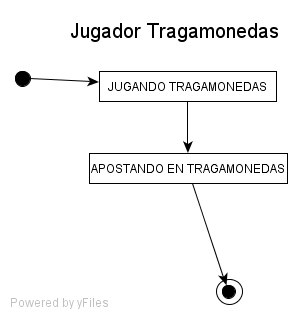
\includegraphics[scale=0.5]{img/JugadorTragamonedasDA.png}
\end{center}

Cada una de estas actividades se explican con mas detalle en los casos de uso: CU \jtra \ref{ljtra} y CU \apotra \ref{lapotra}

%----------------------------------------------------------
% CASO DE USO JUGANDO TRAGAMONEDAS
%----------------------------------------------------------
\label{ljtra}
\begin{cu}{\jtra}
	\descripxizq=1cm
		\defln{Este caso de uso explica como un \jutra que ha ingresado en el casino puede jugar en una mesa de tragamonedas}
		\actor{\jutra}
		\pre{El \jutra debe estar dentro del casino y no estar jugando en ninguna otra mesa}
		\post{El \jutra ha jugado al tragamonedas y ha salido del juego, si ha resultado ganador se modifica su saldo}

\begin{cursoe}{}
	
		\paso{1 El \jutra selecciona el valor de la ficha de la nueva mesa de tragamonedas}{}
		
		\paso{2 El sistema crea una nueva mesa para el \jutra}{}
			
		\paso{3 El sistema informa que el jugador ha ingresado a una mesa de tragamonedas.}{}
		
		\paso{4 El jugador apuesta \incl {\apotra}}{}
				
		\paso{5 El \jutra decide comenzar la jugada }{5.1 Error, la apuesta no es valida, ir a 11}
		
		\paso{6 El sistema da comienzo al juego }{}	
		
		\paso{7 El sistema informa si la jugada es normal, feliz o todos ponen}{}	
	  
	  \paso{8 El sistema muestra el resultado del juego}{}
	  
	  \paso{9 Si el resultado es ganador el sistema acredita el premio correspondiente }{}
	  
	  \paso{10 Si el jugador desea seguir jugando ir a paso 4}{}
	  
	  \paso{11 Sino el sistema automaticamente cierra la mesa}{}
	  
		\paso{12 Fin C.U.}{}
		
  \end{cursoe}

\end{cu}

%-------------------------------
%CASO DE USO APOSTANDO EN TRAGAMONEDAS
%--------------------------------
\label{lapotra}
\begin{cu}{\apotra}
	\descripxizq=1cm
		\defln{Este caso de uso explica como un \aptra apuesta en una mesa Tragamonedas }
		\actor{\apotra}
		\pre{El \jutra debe haber ingresado a una mesa Tragamonedas}
		\post{El \apotra ha apostado en el tragamonedas, y su saldo ha sido modificado }

	\begin{cursoe}{}
    \paso{1 El \apotra selecciona la cantidad de fichas a apostar (entre las permitidas) }{}
		
		\paso{2 Si el \apotra no es VIP el sistema verifica si tiene saldo suficiente para la apuesta}{}
			
		\paso{3 El sistema valida la apuesta y descuenta el monto del saldo del jugador}{3.1 Error: El sistema informa que no tiene saldo suficiente para realizar esta apuesta. Ir a Fin C.U.}
				
		\paso{4 El sistema incrementa el pozo "Premio Gordo Progresivo" }{}
		
		\paso{5 Fin C.U.}{}	
		
	\end{cursoe}
\end{cu}
		

\begin{framed}

\depto Con esta maquina de estados finitos (FSM) mostramos el desarrollo del juego tragamonedas, modelando solo la parte de cobrar o no. 
\\
{\large FSM: JugadaTragamonedas}
\begin{center}
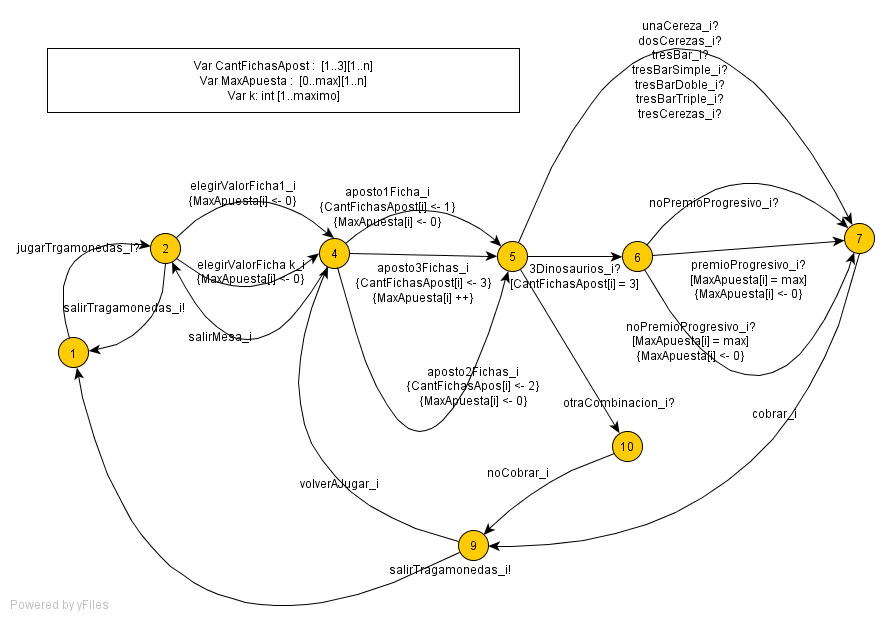
\includegraphics[scale=0.5]{img/JugadaTragamonedas.png}
\end{center}

{\large FSM: MaquinaTragamonedas}
\begin{center}
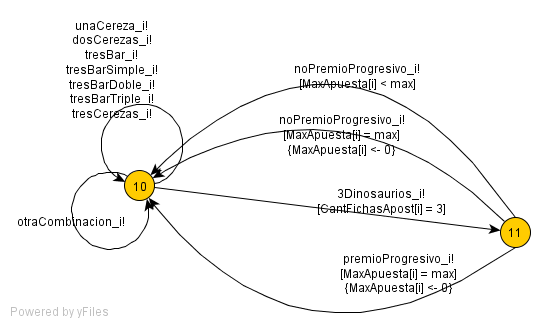
\includegraphics[scale=0.5]{img/MaquinaTragamonedas.png}
\end{center}

\textit{\textsl{Aclaraciones}}: 
\begin{itemize}
	\item{Dado que al abrir el casino se determina con que fichas se jugar�,\textit{\textbf{elegirValorFicha}} refiere a una de esas 	fichas. Es decir, que al abrir una mesa se debe elegir una ficha dentro de las posibles. }
	\item{Abuso de la notacion al referimos a los posibles resultado.}
	\item{Hay tantas FSM maquina tragamonedas como mesas se abran. Cuando
	el jugador sale de la mesa, esta queda inhabilitada para una proxima jugada}
	\item{De haber varias jugadas con posibilidad de ganar el premio progresivo, 	este ser� otorgado solo a una de ellas. 	En la FSM \textit{\textbf{JugadaTragamonedas}} se ve la flecha \textit{\textbf{nopremioProgresivo}} donde la apuesta es maxima, la cual refleja lo explicado previamente}
	\item{Si la apuesta es maxima la cantidad de apuestas de 3 fichas volver� a cero, tanto si gana el premio progresivo 	  o no lo gane}
\end{itemize}

\end{framed}

\subsection{Juego Craps}

Otro de los juegos elegidos por los socios es el \textbf{Craps}. En este juego un tirador lanza un par de dados para establecer un PUNTO y las apuestas girar�n en base a las posibilidades de que dicho tirador repita el mismo punto antes de lanzar un 7.
Cuando un jugador Craps decida jugar debe seleccionar una mesa existente o abrir una nueva. Luego durante el juego podra tirar los dados y/o apostar.

Cada una de estas actividades se explican con mas detalle en los casos de uso: \\
CU \incr \ref{lincr}, CU \jcr \ref{ljcr}, CU \apcr \ref{lapcr} y CU \scr \ref{lscr}

\vskip2cm
%----------------------------------------------------------
% CASO DE USO Ingresando a la mesa de craps
%----------------------------------------------------------
\label{lincr}
\begin{cu}{\incr}
	\descripxizq=1cm
		\defln{Este caso de uso explica como un jugador puede unirse o abrir una nueva mesa de craps }
		\actor{\jucr}
		\pre{El \jucr debe estar dentro del casino y no estar jugando en ninguna otra mesa}
		\post{El \jucr ha ingresado en una mesa de Craps }

	\begin{cursoe}{}
		
		\paso{1 Si hay mesas disponibles el sistema pregunta si el \jucr desea unirse a una mesa, sino hay mesas disponibles ir a paso 3}{}
		
		\paso{2 Si el jugador decide unirse a una mesa selecciona la mesa a la cual desea unirse. Ir a 4}{}
		
		\paso{3 El sistema crea una nueva mesa para el \jucr }{}
		
		\paso{4 El sistema informa que el jugador ha ingresado a una mesa de Craps.}{}
		
	  \paso{5 Fin C.U.}{}
		
	\end{cursoe}
	
\end{cu}

%----------------------------------------------------------
% CASO DE USO Jugando Craps
%----------------------------------------------------------
\label{ljcr}
\begin{cu}{\jcr}
	\descripxizq=1cm
		\defln{Este caso de uso explica como un jugador juega en una nueva mesa de craps }
		\actor{\jucr}
		\pre{El \jucr debe estar dentro del casino y haber ingresado en una mesa de Craps}
		\post{El \jucr ha jugado Craps }

	\begin{cursoe}{}
		
		\paso{1 Si el \jucr desea apuesta. \exti{\apcr}}{}
		
		\paso{2 Si es su turno tira los dados sino observa el resultado}{2.1 Error: La apuesta no es valida por falta de saldo. Ir a 4}%lo mande a ese paso xq si era el unico jugador
		%y no tiene saldo el sistema va a mostrar un resultado "nulo" hasta q se aburra
		
		\paso{3 El sistema informa si la jugada es normal, feliz o todos ponen}{}
				
		\paso{4 El sistema muestra los resultados}{}
		
	  \paso{5 Si el \jucr ha ganado alguna apuesta el sistema acredita el premio correspondiente}{}
	  
	  \paso{6 El sistema modifica el saldo del \jucr si corresponde}{}
	  
	  \paso{7 Si no desea seguir jugando el sistema informa que perdera todas las apuestas  que tenga activas.}{}
% Chicos: lo puse en este orden xq capaz despues de avisarle q pierde sus apuestas si se retira, se arrepiente y en el paso 8 puede optar x seguir, pero si no les gusta lo pueden varia	  
	  \paso{8 Si el jugador desea seguir jugando ir a 1 }{}
	  
	  \paso{9 Sino el sistema saca de la mesa de Craps al \jucr. Incluye saliendo craps }{}
	  
	  \paso{10 Fin C.U.}{}
		
	\end{cursoe}
	
\end{cu}

%-------------------------------
%CASO DE USO APOSTANDO EN CRAPS
%--------------------------------
\label{lapcr}

\begin{cu}{\apcr}
	\descripxizq=1cm
		\defln{Este caso de uso explica como un \apocr apuesta en una mesa de Craps }
		\actor{\apocr}
		\pre{El \apocr debe haber ingresado a una mesa Craps}
		\post{El \apocr ha apostado en el Craps, y su saldo ha sido modificado }

	\begin{cursoe}{}
    \paso{1 El \apocr un tipo de apuesta }{}
    
    \paso{2 El sistema valida el tipo de apuesta }{2.1 Error, el tipo de apuesta no es v�lido para este tiro. Ir a paso 1}
%Con esto quiero decir que si no se ha fijado ya el punto entonces ciertos tipos de apuestas no ser�n v�lidos para esta jugada
    
    \paso{3 El \apocr un monto a apostar}{}
		
		\paso{4 Si el \apocr no es VIP el sistema verifica si tiene saldo suficiente para la apuesta}{}
			
		\paso{5 El sistema valida la apuesta y descuenta el monto del saldo del jugador}{5.1 Error: El sistema informa que no tiene saldo suficiente para realizar esta apuesta. Ir a Fin C.U.}
				
		\paso{6 Si el jugador desea realizar otra apuesta ir a paso 1 }{}
		
		\paso{5 Fin C.U.}{}	
		
	\end{cursoe}
	
\paragraph{Comentario: }
%\begin{flushleft}
%\end{flushleft}
\end{cu}
		
%----------------------------------------------------------
% CASO DE USO Jugando Craps
%----------------------------------------------------------
\label{lscr}
\begin{cu}{\scr}
	\descripxizq=1cm
		\defln{Este caso de uso explica como un jugador sale de una mesa de craps }
		\actor{\jucr}
		\pre{El \jucr debe estar dentro del casino y haber ingresado en una mesa de Craps}
		\post{El \jucr ha salido de una mesa craps }

	\begin{cursoe}{}
		\paso{1 El jugador desea no seguir jugando  }{}
	  
	  \paso{2 El sistema saca de la mesa de Craps al \jucr }{}
	  
	  \paso{3 El sistema cierra automaticamente la mesa si este era el unico jugador en ella}{}	  
	  
	  \paso{4 Fin C.U.}{}

	\end{cursoe}
\end{cu}

\begin{framed}

\depto Con estas maquinas de estados finitos (FSM) mostramos el desarrollo del juego craps. Incluyendo entre ellas un seleccionador, un tirador y cada una de las apuestas. 
\\
{\large FSM: Seleccionador}
\begin{center}
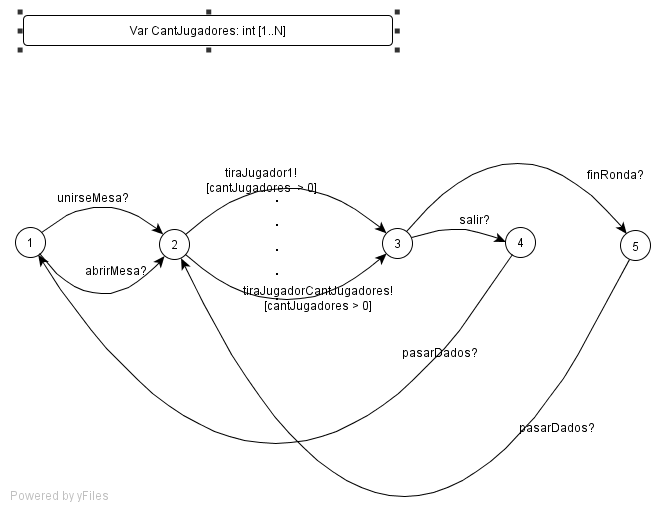
\includegraphics[scale=0.4]{img/seleccionador.png}
\end{center}

Con esta FSM modelamos la eleccion del tirador. 

{\large FSM: Tirador}
\begin{center}
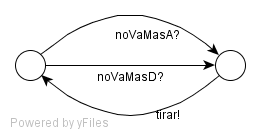
\includegraphics[scale=0.5]{img/tirador.png}
\end{center}

{\large FSM: Cupier}
\begin{center}
%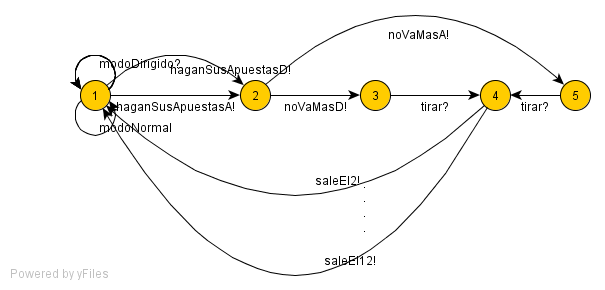
\includegraphics[scale=0.5]{img/coupier.png}
\end{center}



{\large FSM: Jugada Craps}
\begin{center}
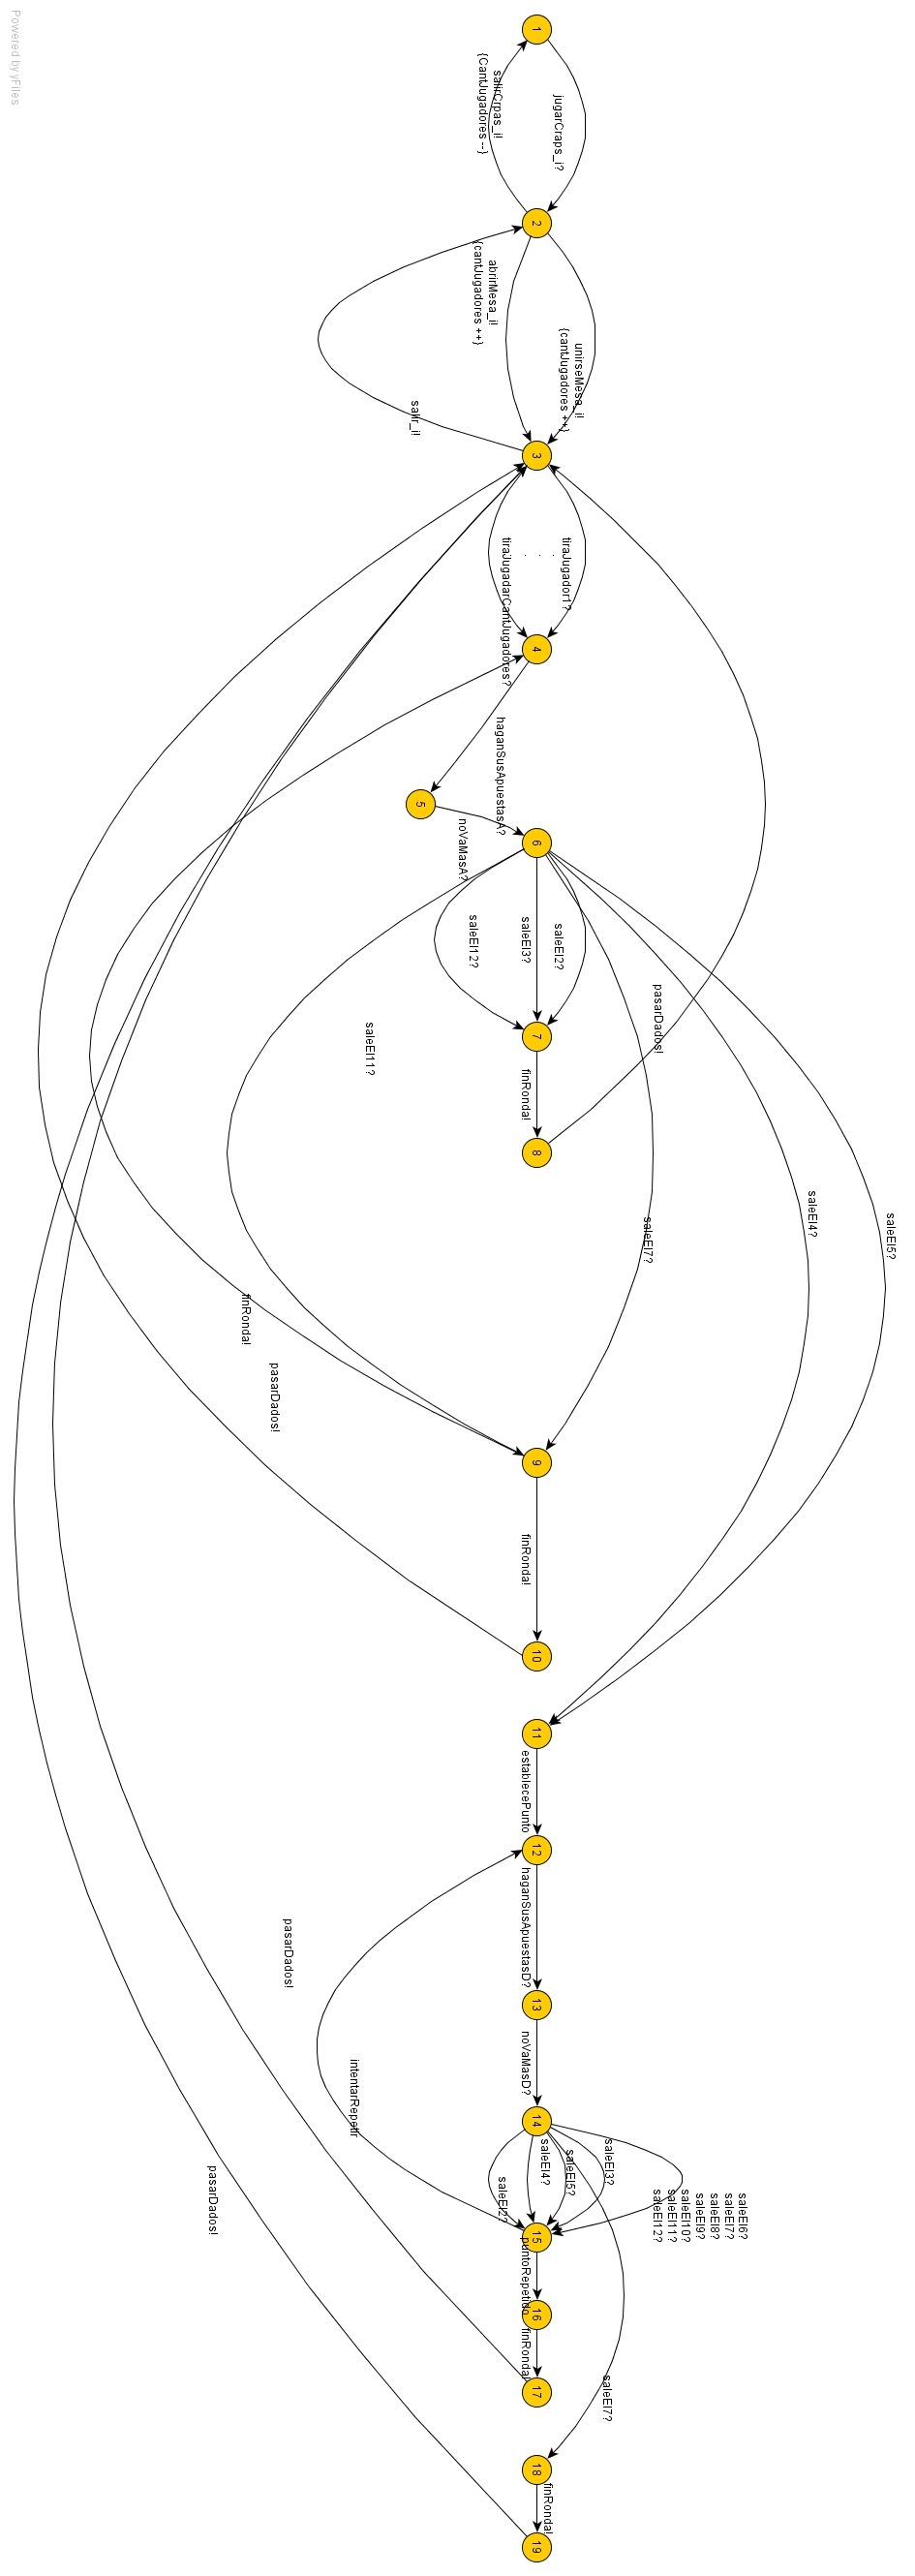
\includegraphics[scale=0.25]{img/desarrolloCraps.png}
\end{center}

Con esta FSM explicamos una jugada de manera general, es decir sin las apuestas. Estas ultimas se explican en el apartado \textit{Pago jugada Craps}. Cabe aclarar que cada una de las apuestas se explican con FSMs distintas; una para cada una de ellas.

\end{framed}


\subsection{Generacion de reportes}

Expicamos en lenguaje OCL como es que se obtienen los datos necesarios para la generacion de los informes.

\subsubsection{Generacion de reporte: Ranking de Jugadores}

\begin{framed}
\begin{lstlisting}[breaklines=true]
--este operacion devuelve dado un jugador una tupla con su nombre y su ganancia
dameNombreGanancia(j:Jugador):TupleType(nombre:String , ganancia: Numero))
pre:	true
post:	result = Tuple{nombre:String = j.nombre, ganancia:Numero = (j.saldo - j.saldoInicial)}


--genera el reporte de ganancia por jugador
--
--busco el jugador que mas gano
--y selecciono todos los jugadores que hayan ganado tanto como el que mas gano
--luego los transforno en tuplas
--
reporteRanking(ascendente:Boolean):Collection(TupleType(nombre:String , ganancia: Numero))
pre:	true
post:	
	let jugadores:Collection(Jugador) = Jugador.allInstances()
	let masGanadores = jugadores->orderedBy(j | j.saldo - j.saldoInicial)
	let menosGanadores = jugadores->orderedBy(j | j.saldoInicial - j.saldo)

if ascendente
then
	result = masGanadores->iterate(j;res=orderedSet();res->including(dameNombreGanancia(j))
else
	result = menosGanadores->iterate(j;res=orderedSet();res->including(dameNombreGanancia(j))
endif

\end{lstlisting}
\end{framed}

\subsubsection{Generacion de reporte: Estado Actual}

\begin{framed}
\begin{lstlisting}[breaklines=true]
--este operacion devuelve dado un jugador una tupla con su nombre y su saldo y el del casino
dameNombreSaldo(j:Jugador):TupleType(nombre:String , ganancia: Numero))
pre:	true
post:	result Tuple{nombre:String = j.nombre, saldo:Numero = j.saldo}

estadoActual(): Collection(TupleType(nombre:String , saldo: Numero))
pre:	true
post:	
	let jugadores:Collection(Jugador) = Jugador.allInstances() 
	let casino:Jornada = Jornada.allInstances()->asSecuence->first()

	result jugadores->iterate(j;res=orderedset();res->including(dameNombreGanancia(j))
		->including(Tuple{nombre:String = "Jornada Actual", saldo:Numero = casino.saldo})

\end{lstlisting}
\end{framed}

\subsubsection{Generacion de reporte: Detalle de movimientos por jugador}

Aqui explicamos como se obtiene la info de los movimientos de cada jugador. Por un lado explicamos como obtener la informacion de tragamonedas y por otro la informacion de craps.

La info que obtenemos con este informe es una lista de apuestas finalizadas de un jugador.
Dicha lista contiene la siguiente informacion:

\begin{itemize}
	\item nombre del jugador
	\item juego (Tragamonedas o Craps)
	\item montoApostado
	\item retribucion		
	\item fecha de realizacion de la apuesta		
\end{itemize}


\begin{framed}
\begin{lstlisting}[breaklines=true]

--este operacion devuelve dado un jugador y una apuesta 
--tragamonedas, una tupla con su nombre, juego, mesa, 
--montoApostado y retribucion

dameInfoApuestaTraga(j:Jugador, a:ApuestaTraga):
    TupleType(nombre:String, juego:String, mesa:Numero, 
    monto:Numero, ganancia: Numero, fecha:Fecha)
    
pre:	a.estado == EstadoAp::ganada or ju.estado == EstadoAp::perdida

post:	
       let mesa = a.jugadaTraga.mesaTragamonedas
       let valorApuesta = a.cantmonedas * mesa.valorFicha
       let valorRetribucion = a.retribucion

result Tuple{nombre:String = j.nombre, ''Juego Tragamonedas'', 
    mesa.numeroMesa, valorApuesta, valorRetribucion, a.fecha}

--busco las apuestas terminadas de tragamonedas y 
--obtengo la info necesaria

dameInfoApuestasTraga(j:Jugador):
    Collection(TupleType(nombre:String, juego:String, 
    mesa:Numero, monto:Numero, ganancia: Numero, fecha:Fecha))
    
pre:	true

post:	
       let apuestas:Collection(ApuestaTragamonedas) = j.apuestaTraga
       let apuestasTerminadas = 
           apuestas.select(a| a.estado != EstadoAp:activa)
       let apuestasOrdenadas = 
           apuestasTerminadas->orderedBy(a | a.fecha)
	
	result apuestasOrgenadas->
	   iterate(a;res=orderedSet();res->including(dameInfoApuestaTraga(j,a))

--este operacion devuelve dado un jugador y una apuesta 
--craps, una tupla con su nombre, juego, mesa, 
--montoApostado y retribucion

dameInfoApuestaCraps(j:Jugador, a:ApuestaCraps):
    TupleType(nombre:String, juego:String, mesa:Numero, 
    monto:Numero, ganancia: Numero, fecha:Fecha)
    
pre:	a.estado == EstadoAp::ganada or ju.estado == EstadoAp::perdida

post:	

result Tuple{nombre:String = j.nombre, ''Juego Craps'', 
    a.hechaEn.numeroMesa, a.monto, a.retribucion, a.fecha}

--busco las apuestas terminadas de craps y 
--obtengo la info necesaria

dameInfoApuestasCraps(j:Jugador):
    Collection(TupleType(nombre:String, juego:String, 
    mesa:Numero, monto:Numero, ganancia: Numero, fecha:Fecha))
    
pre:	true

post:	
       let apuestas:Collection(ApuestaCraps) = j.apuestaCraps
       let apuestasTerminadas = 
           apuestas.select(a| a.estado != EstadoAp:activa)
       let apuestasOrdenadas = 
           apuestasTerminadas->orderedBy(a | a.fecha)
	
	result apuestasOrgenadas->
	   iterate(a;res=orderedSet();res->including(dameInfoApuestaCraps(j,a))

\end{lstlisting}
\end{framed}

\subsection{Pago de jugadas y premios}

Se explicaran aqui con detalle como se refleja el pago de apuestas en el modelo propuesto (Modelo de Clases)\\

\textbf{NOTA: } Esta seccion esta dirigida a solo a lectores con conocimientos de modelo de clases conceptuales y OCL. 

\subsubsection{Pago jugada Tragamonedas}


\begin{framed}

\depto Notese que una jugada tragamonedas solo tiene una apuesta que resolver.


\lstset{language=ocl}
\lstset{commentstyle=\textit}
\begin{lstlisting}[frame=trbl]{}

-- esta operacion paga la apuesta de una jugada de tragamonedas
-- dicha apuesta tiene que estar activa (de otro modo ya ha sido 
-- pagada) 
-- Se paga la jugada y se cobran los premios correspondientes
pagarJugadaTraga(j:JugadaTragamonedas):void
pre: j.estado = EstadoAp:activa
post: 
  -- pago resultado jugada y pago pozo progresivo 
  --y reseteo pozo progresivo
  pagarJugadaTragaBasica(j)
  -- cobro porcentaje jugada todos ponen
  cobrarJugadaToposPonen(j)
  -- pago jugada feliz y reseteo pozo feliz
  pagarJugadaFeliz(j)
  
  if damePremioTraga(j) <> 0
  then 
    j.estado = EstadoAp:Ganada
  else
    j.estado = EstadoAp:Perdida
    
  j.apuestaTragamonedas.retribucion = 
      j.hechaPor.saldo - j.hechaPor.saldo@pre


-- si la jugada es todos ponen decremento saldo jugador e 
-- incremento pozo feliz
pagarJugadaFeliz(j:JugadaTragamonedas):void
pre:  j.estado = EstadoAp:activa
post:   let tipoJugada = j.tipoDeJugada

  if tipoJugada.oclisTypeOf(Feliz)
    j.hechaPor.saldo = j.hechaPor.saldo@pre + 
        oclAsType(Feliz).pozoFeliz.monto
    oclAsType(Feliz).pozoFeliz.monto = 0
  endif


-- si la jugada es todos ponen decremento saldo 
-- jugador e incremento pozo feliz
cobrarJugadaToposPonen(j:JugadaTragamonedas):void
pre:  j.estado = EstadoAp:activa
post:  let tipoJugada = j.tipoDeJugada

  if tipoJugada.oclisTypeOf(TodosPonen)
  then 
    j.hechaPor.saldo = 

      j.hechaPor.saldo@pre +
      (damePremioTraga(j) + damePremioProgesivo(j)) * 
      100 / oclAsType(TodosPonen).porcentaje
    
    oclAsType(TodosPonen).pozoFeliz.monto = 

      oclAsType(TodosPonen).pozoFeliz.monto@pre + 
      ((damePremioTraga(j) + damePremioProgesivo(j)) * 
      100 / oclAsType(TodosPonen).porcentaje)
      
  endif



-- incremento saldo jugados de jugada y pozo progresivo 
-- (si corresponde)
-- decremento saldo casino
-- decremento pozo (si corresponde)
pagarJugadaTragaBasica(j:JugadaTragamonedas):void
pre:  j.estado = EstadoAp:activa
post:  
  let jornada = Jornada.allInstances->asSecuence->first()

  j.hechaPor.saldo = j.hechaPor.saldo@pre + 
       (damePremioTraga(j) + damePremioProgesivo(j))
  jornada.saldo = jornada.saldo@pre - cualEsElPrepmio(j)
  if damePremioProgesivo(j) <> 0
  then
    PozoProgresivo.allInstances()->asSecuence()->first().monto = 0
  endif


-- devuelve el valor del premio correspondiente a la jugada
damePremioTraga(j:JugadaTagamonesas):Numero
pre:  
post:  let conjRes:Collection  = 
ResultadoPosibleTagamonedas.allInstances()->select(  r |   
            r.res1 = j.res1 and
            r.res2 = j.res2 and
            r.res3 = j.res2 and
            r.cantMonedas = j.apuestaTragamonesas.cantMonedas) 
  let precioFicha = j.mesaTragamonedas.valorFicha

  if not(conjRes->isEmpty()) then
    result = conjRes->asSecuence()->first().ganMonedas * precioFicha 
  else
    result = 0

  endif 


-- devuelve el valor del premio progresivo 
-- correspondiente a la jugada
damePremioProgesivo(j:JugadaTagamonesas):Numero
pre:  true
post:  let conjRes:Collection  = 
ResultadoPosibleTagamonedas.allInstances()->
	select(r | r.res1 = j.res1 and
            r.res2 = j.res2 and
            r.res3 = j.res2 and
            r.cantMonedas = j.apuestaTragamonesas.cantMonedas) 
  let precioFicha = j.mesaTragamonedas.valorFicha

  if not(conjRes->isEmpty()) then
    if   j.res1 = Fruta::Dinosaurio and
      j.res2 = Fruta::Dinosaurio and
      j.res3 = Fruta::Dinosaurio and
      j.mesaTragamonedas.CantPalancasMax = 3
    then
      result = 
          j.mesaTragamonedas.pozoProgresivo.monto * precioFicha 
    else
      result = 0
    endif
  else
    result = 0
  endif 
  
\end{lstlisting}

\end{framed}


\subsubsection{Pago jugada Craps}

\vskip1cm
\textsc{Explicacion de Apuestas juego Craps}
\vskip1cm

{\large FSM: Linea de Pase}
\begin{center}
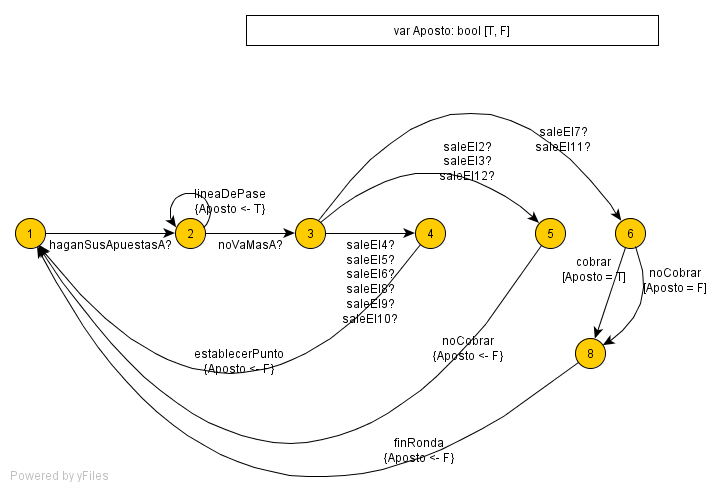
\includegraphics[scale=0.5]{img/linesDePase.png}
\end{center}

{\large FSM: Barra No Pase}
\begin{center}
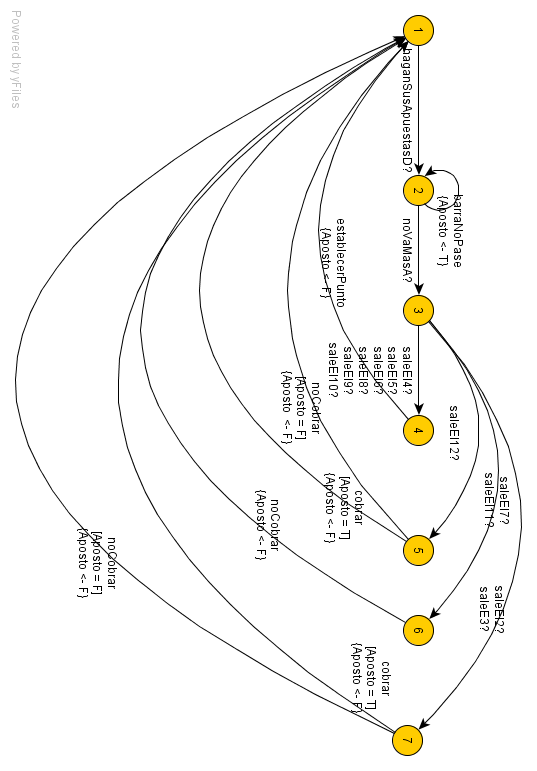
\includegraphics[scale=0.5]{img/barraNoPase.png}
\end{center}

\newpage
{\large FSM: Apuesta Venir }
\begin{center}
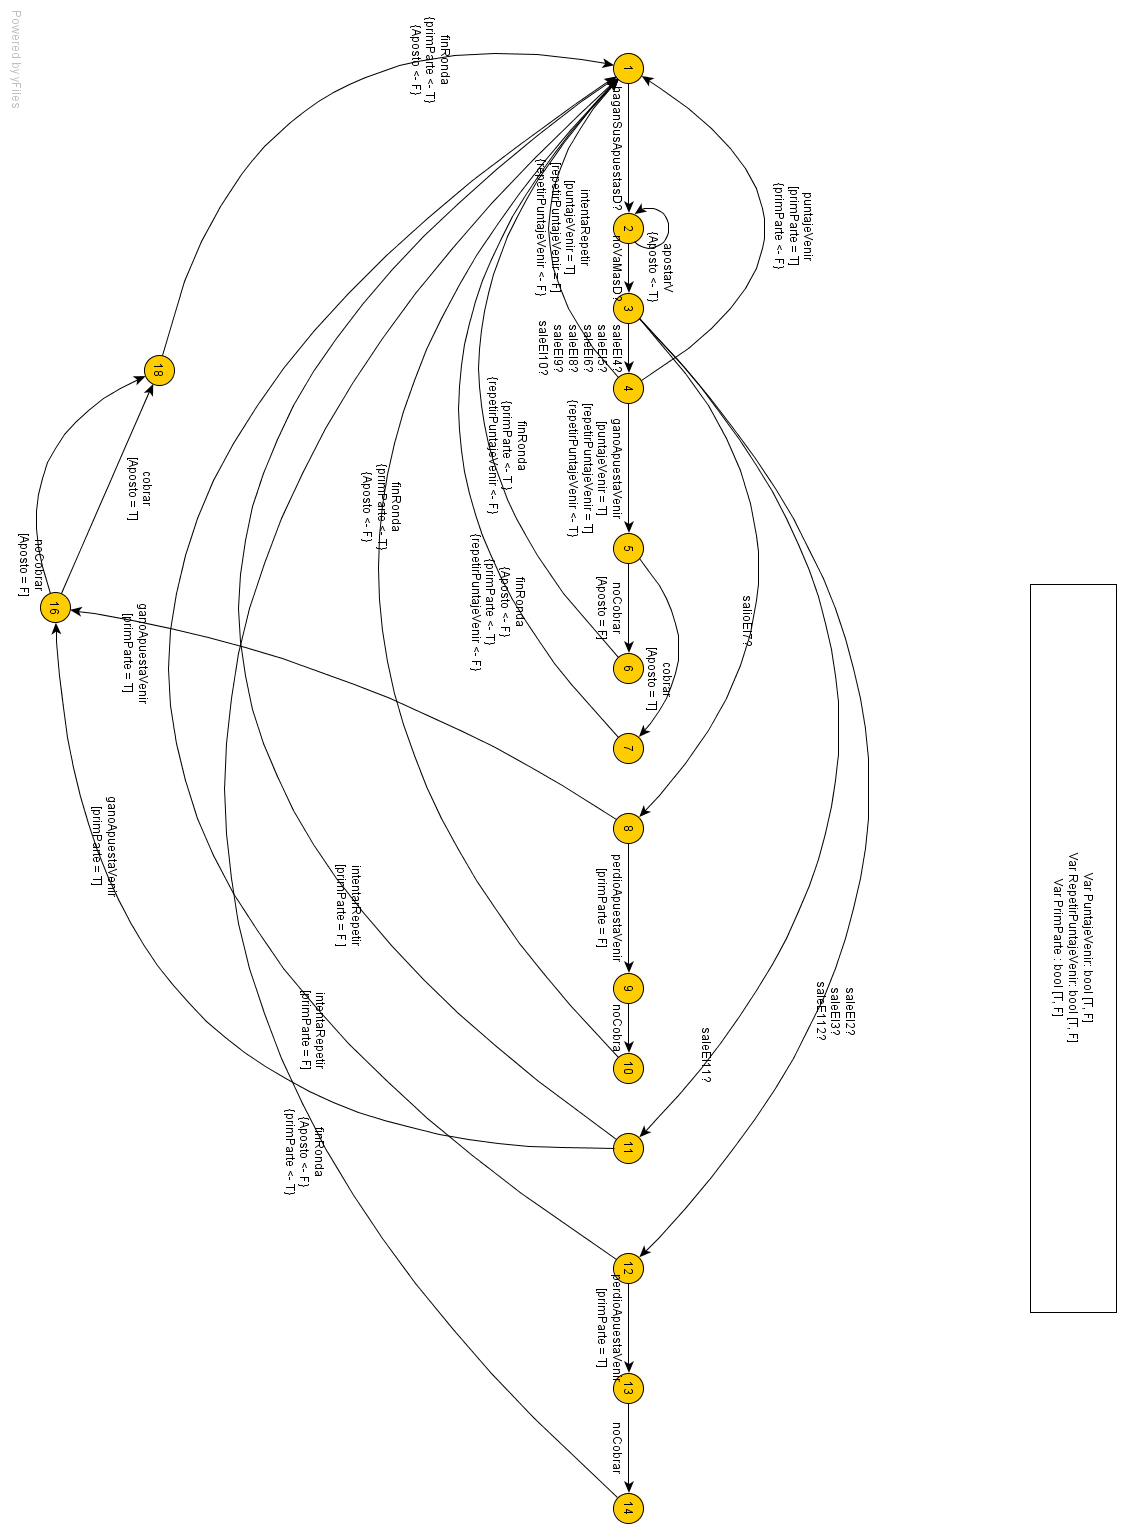
\includegraphics[scale=0.4]{img/ApuestaVenir.png}
\end{center}

\newpage
{\large FSM: Apuesta No Venir}
\begin{center}
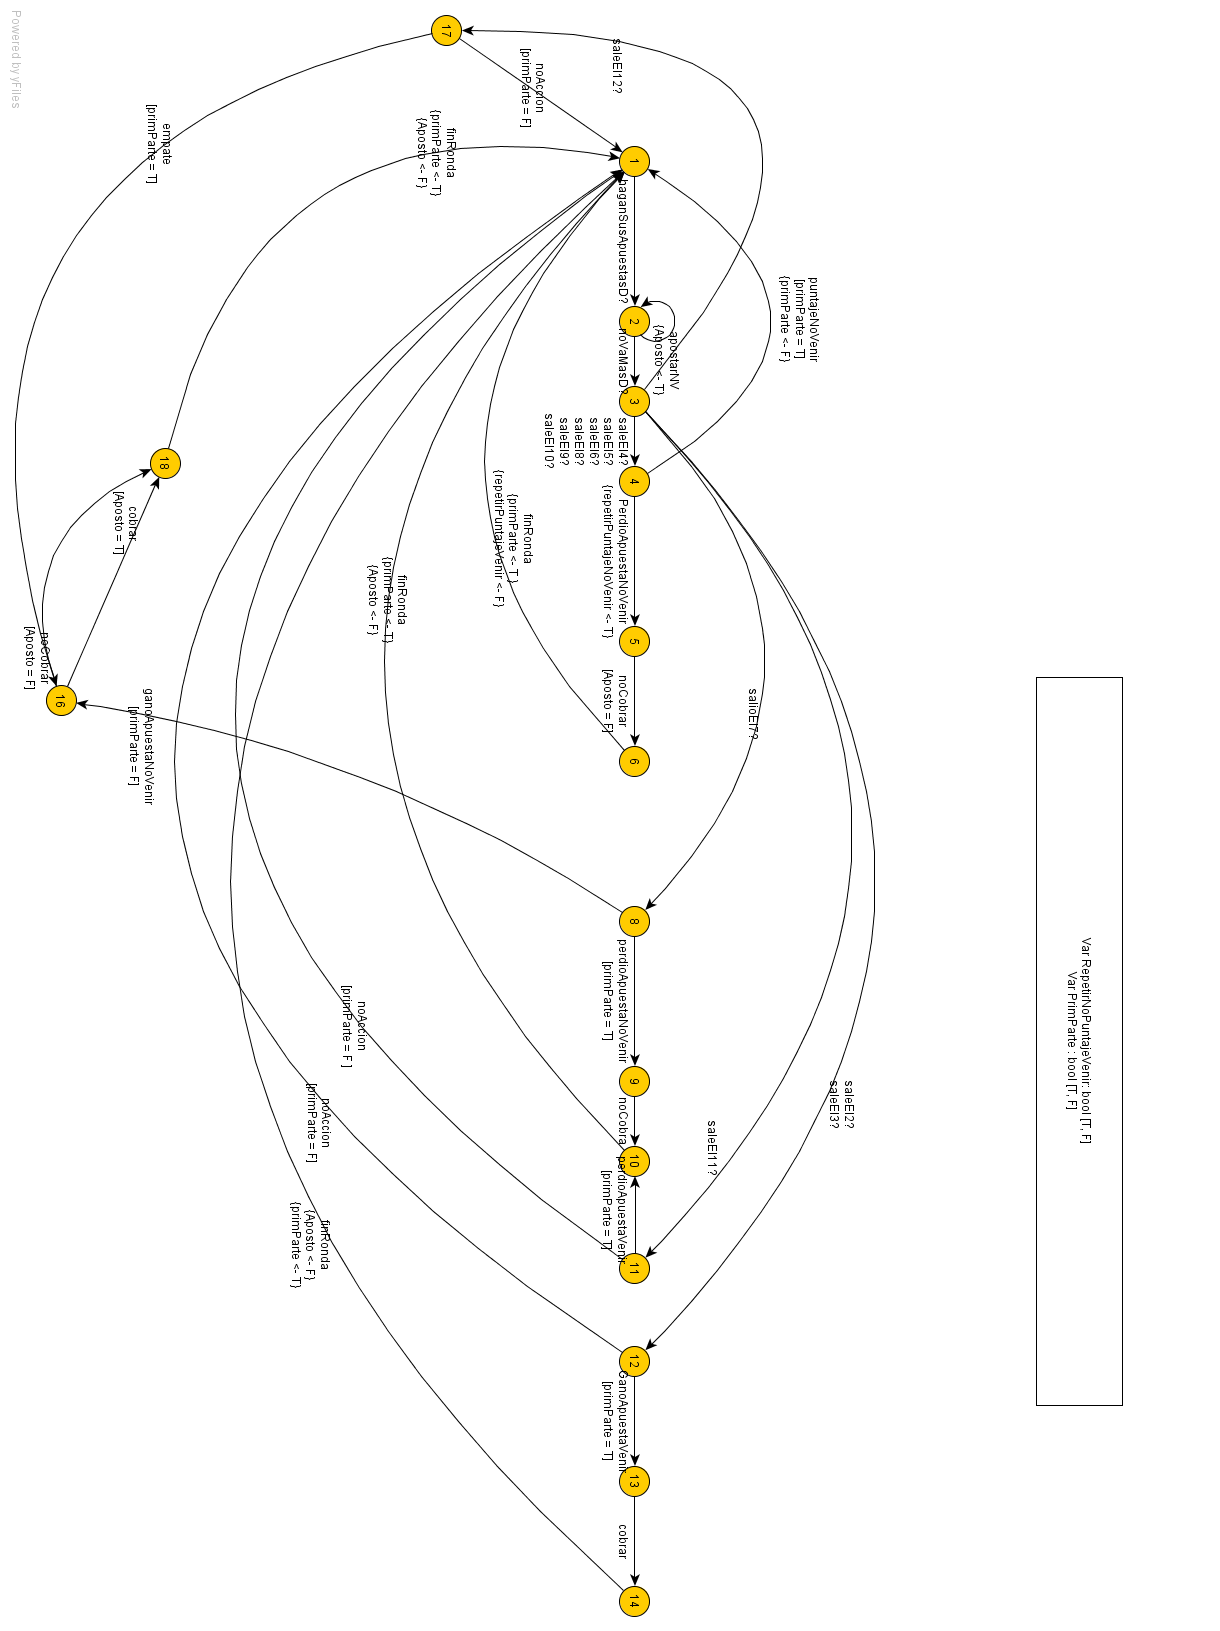
\includegraphics[scale=0.35]{img/apuestaNoVenir.png}
\end{center}

\newpage
{\large FSM: Apuesta De Campo}
\begin{center}
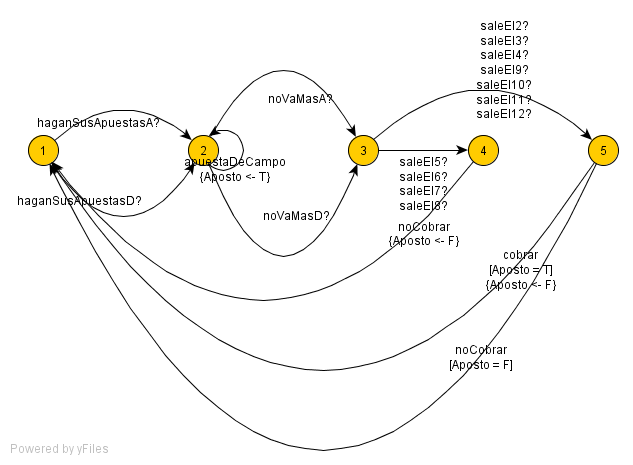
\includegraphics[scale=0.5]{img/apuestaDeCampo.png}
\end{center}

{\large FSM: Apuesta En Sitio}
\begin{center}
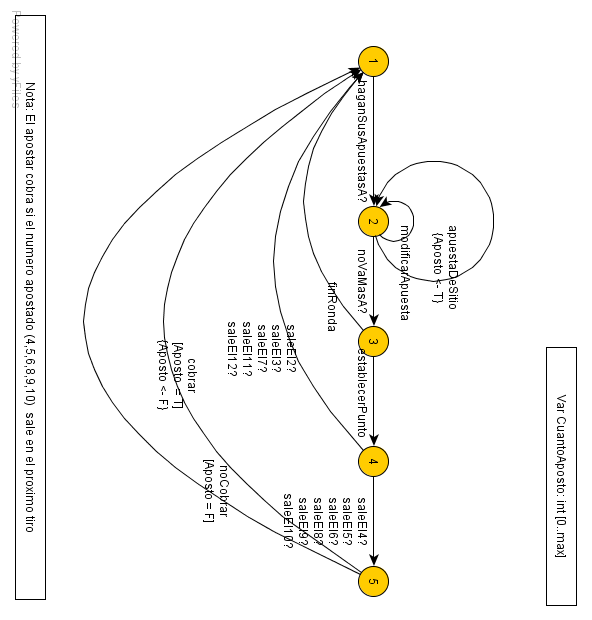
\includegraphics[scale=0.5]{img/apuestaEnSitio.png}
\end{center}

\newpage
{\large FSM: Apuesta a Ganar}
\begin{center}
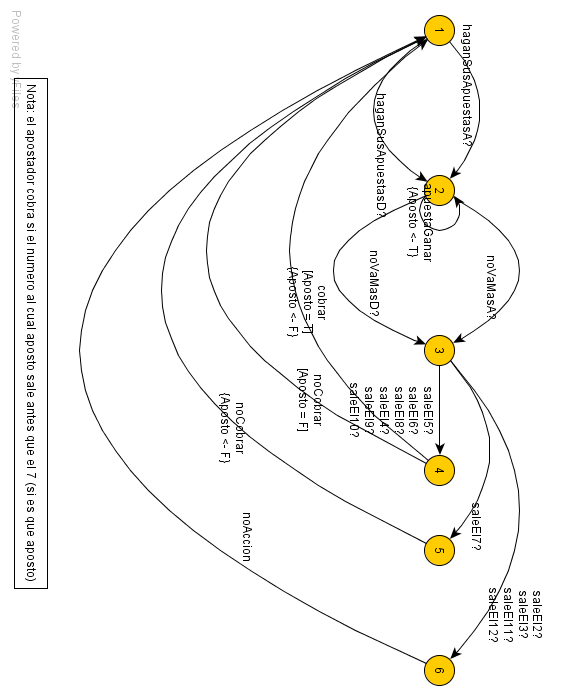
\includegraphics[scale=0.5]{img/apuestaAGanar.png}
\end{center}


{\large FSM: Apuesta En Contra}
\begin{center}
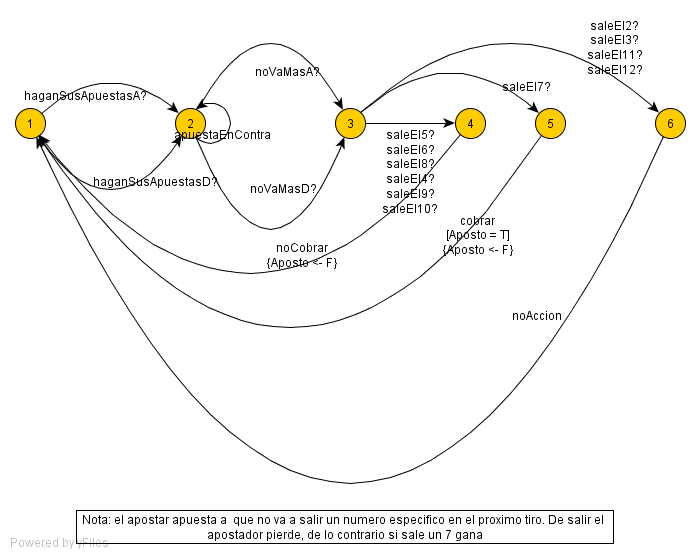
\includegraphics[scale=0.5]{img/apuestaEnContra.png}
\end{center}

%\end{framed}

\vskip1cm
\textsc{Especificacion de Apuestas juego Craps}
\vskip1cm

\begin{framed}
\depto Esta es la operacion que quedo como el TP original que esta ``Harcodeada''. \textbf{SERGIO: } Por lo que hablamos nos permitiste dejarla tal cual estaba.
\end{framed}

\begin{framed}
\begin{lstlisting}[breaklines=true]
pagoApuestaPaseDelinea(j: jugadaCraps, ap: ApuestaCraps, 
   jug:jugador, jorn: Jornada) : void
pre: ap.estado = EstadoAp:Activa and 
     ap.tipo = TipoApCraps:Pase and 
     jug.participaEn.JugadaCraps->exist( y | y = j) 
     and ap.hechaEn.JugadaCraps->exist(t | t = ap)
post:

  if (j.resultado = 7 or j.resultado = 11) then
    ap.estado = EstadoAp:ganada

    //jugada todos ponen
    if ( tipoJugada.oclisTypeOf(TodosPonen)) then 
    
    jug.saldo = jug.saldo@pre + (ap.retribucion *  100 / oclAsType(TodosPonen).porcentaje)
    
    oclAsType(TodosPonen).pozoFeliz.monto = oclAsType(TodosPonen).pozoFeliz.monto@pre + 
          (ap.retribucion *  100 / oclAsType(TodosPonen).porcentaje)

    jorn.saldo = jorn.saldo@pre - (ap.retribucion *  100 / oclAsType(TodosPonen).porcentaje)

    
    else
    //jugada normal
    jug.saldo = jug.saldo@pre + ap.retribucion
    jorn.saldo = jorn.saldo@pre - ap.retribucion

    endif
  else 
    if (j.resultado = 2 or j.resultado = 3 or j.resultado = 12) then
      ap.estado = EstadoAp:perdida
      jug.saldo = jug.saldo@pre - ap.apuesta.
      jorn.saldo = jorn.saldo@pre + ap.apuesta
  
    end if
  endif


----------------------------------------------------------------    
pagoApuestaNoPase(j: jugadaCraps, ap: ApuestaCraps, jug:jugador, jorn: Jornada) : void
pre: ap.estado = EstadoAp:Activa and ap.tipo = TipoApCraps:NoPase and jug.participaEn.JugadaCraps->exist( y | y = j) 
     and ap.hechaEn.JugadaCraps->exist(t | t = ap)
post:

  if (j.resultado = 2 or j.resultado = 3) then
    ap.estado = EstadoAp:ganada

    //jugada todosponen
    if ( tipoJugada.oclisTypeOf(TodosPonen)) then 
    
    jug.saldo = jug.saldo@pre + (ap.retribucion *  100 / oclAsType(TodosPonen).porcentaje)
    
    oclAsType(TodosPonen).pozoFeliz.monto = oclAsType(TodosPonen).pozoFeliz.monto@pre + 
          (ap.retribucion *  100 / oclAsType(TodosPonen).porcentaje)

    jorn.saldo = jorn.saldo@pre - (ap.retribucion *  100 / oclAsType(TodosPonen).porcentaje)

    else

    //jugada normal
    jug.saldo = jug.saldo@pre + ap.retribucion
    jorn.saldo = jorn.saldo@pre - ap.retribucion

    endif

  else 
    if (j.resultado = 7 or j.resultado = 11 )then
      ap.estado = EstadoAp:perdida
      jug.saldo = jug.saldo@pre - ap.apuesta.
      jorn.saldo = jorn.saldo@pre + ap.apuesta
    endif
  
  endif

-----------------------------------------------------------------
pagoApuestaVenir(j: jugadaCraps, ap: ApuestaCraps, jug:jugador, jorn: Jornada) : void
pre: ap.estado = EstadoAp:Activa and ap.tipo = TipoApCraps:Venir and jug.participaEn.JugadaCraps->exist( y | y = j) 
     and ap.hechaEn.JugadaCraps->exist(t | t = ap)
post:

  if (j.resultado = 7 or j.resultado = 11) then
    ap.estado = EstadoAp:ganada

    //jugada todosponen
    if ( tipoJugada.oclisTypeOf(TodosPonen)) then 
    
    jug.saldo = jug.saldo@pre + (ap.retribucion *  100 / oclAsType(TodosPonen).porcentaje)
    
    oclAsType(TodosPonen).pozoFeliz.monto = oclAsType(TodosPonen).pozoFeliz.monto@pre + 
          (ap.retribucion *  100 / oclAsType(TodosPonen).porcentaje)

    jorn.saldo = jorn.saldo@pre - (ap.retribucion *  100 / oclAsType(TodosPonen).porcentaje)

    else

    //jugada normal


    jug.saldo = jug.saldo@pre + ap.retribucion
    jorn.saldo = jorn.saldo@pre - ap.retribucion

  else 
    if (j.resultado = 2 or j.resultado = 3 or j.resultado = 12 )then
      ap.estado = EstadoAp:perdida
      jug.saldo = jug.saldo@pre - ap.apuesta.
      jorn.saldo = jorn.saldo@pre + ap.apuesta
    endif
  
  endif

--------------------------------------------------------------------
pagoApuestaNoVenir(j: jugadaCraps, ap: ApuestaCraps, jug:jugador, jorn:Jornada) : void
pre: ap.estado = EstadoAp:Activa and ap.tipo = TipoApCraps:NoVenir and jug.participaEn.JugadaCraps->exist( y | y = j) 
     and ap.hechaEn.JugadaCraps->exist(t | t = ap)
post:

  if (j.resultado = 2 or j.resultado = 3) then
    ap.estado = EstadoAp:ganada
    
    //jugada todosponen
    if ( tipoJugada.oclisTypeOf(TodosPonen)) then 
    
    jug.saldo = jug.saldo@pre + (ap.retribucion *  100 / oclAsType(TodosPonen).porcentaje)
    
    oclAsType(TodosPonen).pozoFeliz.monto = oclAsType(TodosPonen).pozoFeliz.monto@pre + 
          (ap.retribucion *  100 / oclAsType(TodosPonen).porcentaje)

    jorn.saldo = jorn.saldo@pre - (ap.retribucion *  100 / oclAsType(TodosPonen).porcentaje)

    else

    //jugada normal


    jug.saldo = jug.saldo@pre + ap.retribucion
    jorn.saldo = jorn.saldo@pre - ap.retribucion

  else 
    if (j.resultado = 7 or j.resultado = 11) then
      ap.estado = EstadoAp:perdida
      jug.saldo = jug.saldo@pre - ap.apuesta.
      jorn.saldo = jorn.saldo@pre + ap.apuesta
    endif
  
  endif

----------------------------------------------------------------------
pagoApuestaDeCampo(j: jugadaCraps, ap: ApuestaCraps, jug:jugador, jorn: Jornada) : void
pre: ap.estado = EstadoAp:Activa and ap.tipo = TipoApCraps:Campo and jug.participaEn.JugadaCraps->exist( y | y = j) 
     and ap.hechaEn.JugadaCraps->exist(t | t = ap)
post:
  let loqAposto = ap.valor
  let ganancia =  ap.retribucion

  if(loqAposto = j.resultado) then

    if (loqAposto = 3 or loqAposto = 4 or loqAposto = 9 or loqAposto = 10 or loqAposto = 11)

      ap.estado = EstadoAp:ganada
      
      ganancia = ap.retribucion
    else
      if (loqAposto = 2 or loqAposto = 12) then
      
        ap.estado = EstadoAp:ganada
        
        ganacia = ap.retribucion * 2
        
      endif
    endif
      //jugada todosponen
      if ( tipoJugada.oclisTypeOf(TodosPonen)) then 
    
      jug.saldo = jug.saldo@pre + (ganancia *  100 / oclAsType(TodosPonen).porcentaje)
    
      oclAsType(TodosPonen).pozoFeliz.monto = oclAsType(TodosPonen).pozoFeliz.monto@pre + 
            (ap.retribucion *  100 / oclAsType(TodosPonen).porcentaje)

      jorn.saldo = jorn.saldo@pre - (ganancia *  100 / oclAsType(TodosPonen).porcentaje)

      else

      //jugada normal


      jug.saldo = jug.saldo@pre + ganancia
      jorn.saldo = jorn.saldo@pre - ganancia  


  else 
    
    ap.estado = EstadoAp:perdida
    jug.saldo = jug.saldo@pre - ap.apuesta.
    jorn.saldo = jorn.saldo@pre + ap.apuesta
    
  
  endif

----------------------------------------
pagoApuestaDeSitio(j: jugadaCraps, ap: ApuestaCraps, jug:jugador, jorn: Jornada) : void
pre: ap.estado = EstadoAp:Activa and ap.tipo = TipoApCraps:Sitio and jug.participaEn.JugadaCraps->exist( y | y = j) 
     and ap.hechaEn.JugadaCraps->exist(t | t = ap)
post: let loqAposto = ap.valor

  if (j.resultado = 4 or j.resultado = 5 or j.resultado = 6 or j.resultado = 8 or j.resultado = 9 or j.resultado = 10) then

    if ( j.resultado = ap.valor) then
      
       ap.estado = EstadoAp:ganada
      //jugada todosponen
      if ( tipoJugada.oclisTypeOf(TodosPonen)) then 
    
      jug.saldo = jug.saldo@pre + (ap.retribucion *  100 / oclAsType(TodosPonen).porcentaje)
    
      oclAsType(TodosPonen).pozoFeliz.monto = oclAsType(TodosPonen).pozoFeliz.monto@pre + 
            (ap.retribucion *  100 / oclAsType(TodosPonen).porcentaje)

      jorn.saldo = jorn.saldo@pre - (ap.retribucion *  100 / oclAsType(TodosPonen).porcentaje)

      else

      //jugada normal


      jug.saldo = jug.saldo@pre + ap.retribucion
      jorn.saldo = jorn.saldo@pre - ap.retribucion

 
    else
      
      ap.estado = EstadoAp:perdida
      jug.saldo = jug.saldo@pre - ap.apuesta.
      jorn.saldo = jorn.saldo@pre + ap.apuesta

    endif


  endif

-------------------------------------------


pagoApuestaGanar(j: jugadaCraps, ap: ApuestaCraps, jug:jugador, jorn: Jornada) : void
pre: ap.estado = EstadoAp:Activa and ap.tipo = TipoApCraps:Ganar and jug.participaEn.JugadaCraps->exist( y | y = j) 
     and ap.hechaEn.JugadaCraps->exist(t | t = ap)
post: let loqAposto = ap.valor
  let cantFichasApost = ap.
  let ganancia = ap.retribucion

  if (j.resultado = 7) then

      ap.estado = EstadoAp:perdida
      jug.saldo = jug.saldo@pre - ap.apuesta.
      jorn.saldo = jorn.saldo@pre + ap.apuesta

  else

   if (j.resultado = 4 or j.resultado = 5 or j.resultado = 6 or j.resultado = 8 or j.resultado = 9 or j.resultado = 10) then


            if (j.resultado = loqAposto and loqAposto = 4)

      ap.estado = EstadoAp:ganada
      if ( ap.apuesta mod 5 = 0) then
      ganancia = ap.retribucion + 9* ap.retribucion
      
      else
      
      ganancia = ap.retribucion 
      
       if (j.resultado = loqAposto and loqAposto = 5)

      ap.estado = EstadoAp:ganada
      if ( ap.apuesta mod 5 = 0) then
      
      ganancia = ap.retribucion + 8 * ap.retribucion
      
      else
      ganancia = ap.retribucion 
        

        if (j.resultado = loqAposto and loqAposto = 6)

      ap.estado = EstadoAp:ganada
      if ( ap.apuesta mod 6 = 0) then
      ganancia = ap.retribucion + 7 * ap.retribucion
      
      
      else
      ganancia = ap.retribucion 
      

         if (j.resultado = loqAposto and loqAposto = 8)

      ap.estado = EstadoAp:ganada
      if ( ap.apuesta mod 6 = 0) then
      ganancia = ap.retribucion + 7 * ap.retribucion
      

      else
      ganancia = ap.retribucion 
      

                      if (j.resultado = loqAposto and loqAposto = 9)

      ap.estado = EstadoAp:ganada
      if ( ap.apuesta mod 5 = 0) then
      ganancia =  ap.retribucion + 7 * ap.retribucion
      

      else
      ganancia + ap.retribucion 
      


          if (j.resultado = loqAposto and loqAposto = 10)

      ap.estado = EstadoAp:ganada
      if ( ap.apuesta mod 5 = 0) then
      ganancia = ap.retribucion + 9 * ap.retribucion
      

      else
      ganancia = + ap.retribucion 
    

          //jugada todosponen
      if ( tipoJugada.oclisTypeOf(TodosPonen)) then 
    
      jug.saldo = jug.saldo@pre + (ganancia *  100 / oclAsType(TodosPonen).porcentaje)
    
      oclAsType(TodosPonen).pozoFeliz.monto = oclAsType(TodosPonen).pozoFeliz.monto@pre + 
            (ap.retribucion *  100 / oclAsType(TodosPonen).porcentaje)

      jorn.saldo = jorn.saldo@pre - (ganancia *  100 / oclAsType(TodosPonen).porcentaje)

      else

      //jugada normal


      jug.saldo = jug.saldo@pre + ganancia
      jorn.saldo = jorn.saldo@pre - ganancia  
      
  


   endif

-----------------------------------------------------
pagoApuestaenContra(j: jugadaCraps, ap: ApuestaCraps, jug:jugador, jorn: Jornada) : void
pre: ap.estado = EstadoAp:Activa and ap.tipo = 
  TipoApCraps:Contra and jug.participaEn.JugadaCraps->exist( y | y = j) 
     and ap.hechaEn.JugadaCraps->exist(t | t = ap)
post: let loqAposto = ap.valor
  

  if (j.resultado = 7) then

      ap.estado = EstadoAp:ganada
      
  
            if (loqAposto = 4)

      
      if ( ap.apuesta mod 11 = 0) then
      ganancia =  ap.retribucion + 5* ap.retribucion
      
      else
      
      ganancia = ap.retribucion 
      
     if (loqAposto = 5)

      if ( ap.apuesta mod 8 = 0) then
      ganancia = ap.retribucion + 5* ap.retribucion
      
      else
      
      ganancia = ap.retribucion 
      

     if (loqAposto = 6)


                        if ( ap.apuesta mod 5 = 0) then
      ganancia = ap.retribucion + 4* ap.retribucion
      
      else
      
      ganancia = ap.retribucion 
      
                 if (loqAposto = 9)

                         if ( ap.apuesta mod 8 = 0) then
      ganancia = ap.retribucion + 5* ap.retribucion
      
      else
      
      ganancia = ap.retribucion 
      
     if (loqAposto = 10)

                        if ( ap.apuesta mod 11 = 0) then
      ganancia = ap.retribucion + 5* ap.retribucion
      
      else
      
      ganancia = ap.retribucion 
      
    //jugada todosponen
      if ( tipoJugada.oclisTypeOf(TodosPonen)) then 
    
      jug.saldo = jug.saldo@pre + (ganancia *  100 / oclAsType(TodosPonen).porcentaje)
    
      oclAsType(TodosPonen).pozoFeliz.monto = oclAsType(TodosPonen).pozoFeliz.monto@pre + 
            (ap.retribucion *  100 / oclAsType(TodosPonen).porcentaje)

      jorn.saldo = jorn.saldo@pre - (ganancia *  100 / oclAsType(TodosPonen).porcentaje)

      else

      //jugada normal


      jug.saldo = jug.saldo@pre + ganancia
      jorn.saldo = jorn.saldo@pre - ganancia  
  

  else

    ap.estado = EstadoAp:perdida
    jug.saldo = jug.saldo@pre - ap.apuesta.
    jorn.saldo = jorn.saldo@pre + ap.apuesta.


  endif
\end{lstlisting}  

\end{framed}